\documentclass{article}

\usepackage[a4paper, total={6in, 8.6in}]{geometry}
% \usepackage[utf8]{inputenc}

\usepackage{amsmath}
\usepackage{amssymb}
\usepackage{amsthm}
\usepackage{xcolor}
\usepackage{mathtools}

% for feynman diagrams
\usepackage{fontspec}
\usepackage{tikz}
\usetikzlibrary{decorations.markings}
\usetikzlibrary{arrows.meta}
\usepackage[compat=1.1.0]{tikz-feynman}

\usepackage{bbm} % blackboard bold '1'

\usepackage{hyperref}

\DeclarePairedDelimiter{\floor}{\lfloor}{\rfloor}
\newcommand{\dx}{\mathrm{d}}

\newtheorem{theorem}{Theorem}[section]
\newtheorem{corollary}{Corollary}[theorem]
\newtheorem{proposition}[theorem]{Proposition}
\newtheorem{lemma}[theorem]{Lemma}
\theoremstyle{definition}
\newtheorem{definition}{Definition}[section]
\theoremstyle{remark}
\newtheorem{remark}{Remark}
\theoremstyle{remark}
\newtheorem{example}{Example}

% Bibliography setup
\usepackage[backend=biber]{biblatex}
\addbibresource{refs.bib}

\title{Super interesting title on weakly interacting fermionic systems}
\author{Filippo Cozzi}
\date{???}


\begin{document}

\maketitle
\tableofcontents

\section{Second Quantization}

\textcolor{red}{INTROOOOO}

\subsection{Principles of quantum mechanics}

\subsection*{Preliminaries}

In this preliminary section we give an overvew of the mathematical objects that appear in the
description of quantum systems. The probabilistic nature of a quantum system is realized in
the linear structure of a complex vector space that is equipped with an inner product, which
produces the probability amplitude for a system prepared in some state to be measured in
another. In this setting, linear combinations of state vectors are just probabilistic
superpositions. We will give the necessary definitions regarding a particular class of vector
spaces, even though many concepts come from more general settings.

\begin{definition}[Hilbert space]
	A (complex) \textit{Hilbert space} $\mathcal{H}$ is a vector space equipped with a
	sesquilinear map $\langle\cdot,\cdot\rangle:\mathcal{H}\times\mathcal{H}\to\mathbb{C}$
	such that $\Vert\phi\Vert\coloneq\langle\phi,\phi\rangle^{1/2}$ defines a norm which makes
	$\mathcal{H}$ a complete metric space.
\end{definition}

A note on the choice of notation. Sometimes, using Dirac's ``bra-ket" notation can help avoid
ambiguities. In this notation, a vector would be denoted by $|\psi\rangle\in\mathcal{H}$, a
linear functional as $\langle\psi|\in\mathcal{H}^*$, and the inner product (with respect to a
symmetric operator, which we haven't yet introduced) as $\langle\psi,A\phi\rangle=\langle\psi|
A|\phi\rangle$. An example of such a scenario where this notation \textit{might} be preferred
is that of the occupation number basis, which we make use of in Chapter (\ref{second-order}).

\begin{definition}
	A Hilbert space is said to be \textit{separable} if it admits a countable dense subset.
\end{definition}

The relevance of this definition stems from the fact that, if we can find a countable set
$\mathcal{S} = \{u_n:n\in\mathbb{N}\}$ of vectors in the Hilbert space $\mathcal{H}$ such that
the space of \textit{finite} linear combinations of elements from $\mathcal{S}$ is dense, we
have that any vector in $\mathcal{H}$ can be expressed as a limit of such finite linear
combinations. That is, the set $\mathcal{S}$ is \textit{complete} (acts as a \textit{basis})
in the sense that, ignoring problems with linear independence, any vector can be identified
with a sequence of components $\{a_n:n\in\mathbb{N}\}$, with the condition that the series
$\sum_{n\in\mathbb{N}}a_n u_n$ converges (in the norm topology of $\mathcal{H}$). When
speaking of Hilbert spaces we will always assume that they are separable.

\begin{lemma}
	If $X$ is a dense subspace of the Hilbert space $\mathcal{H}$, it is always possible to
	choose a complete orthonormal system $\{u_n:n\in\mathbb{N}\}$ for $\mathcal{H}$ composed
	only of elements in $X$.
\end{lemma}
\begin{proof}
	Since $\overline{X}=\mathcal{H}$, for all $x\in\mathcal{H}$ there exists a sequence $\{x_n
	\}_{n\in\mathbb{N}}\subseteq X$ such that $x_n\to x$. Let $\{y_n\}_{n\in\mathbb{N}}$ be a
	complete orthonormal set for $\mathcal{H}$, then for any $n$ there exists a sequence $\{
	u^{(n)}_m\}_{m\in\mathbb{N}}$ such that $\lim_m u^{(n)}_m = y_n$.
	Define
	\begin{align*}
		\mathcal{S} \coloneq \{ u^{(n)}_m : n,m\in\mathbb{N} \},
	\end{align*}
	which is countable because it is a countable union of countable sets. The set $\mathcal{S}$
	is complete, indeed let $x\in\mathcal{H}$, then there exists a sequence $\{\lambda_m\}_{m
	\in\mathbb{N}}$ such that $\sum_{k=1}^\infty\vert\lambda_k\vert^2<\infty$ and $x=
	\sum_{k=1}^\infty \lambda_k y_k$: we can express $y_k$ as a limit, as discussed above, to
	get that
	\begin{align*}
		x = \sum_{k=1}^\infty \lambda_k y_k
		= \sum_{k=1}^\infty\lambda_k \lim_{m\to\infty}u^{(k)}_m
		= \lim_{m\to\infty}\sum_{k=1}^\infty\lambda_k u^{(k)}_m,
	\end{align*}
	which implies that the sequence $\{\sum_{k=1}^N\lambda_k u^{(k)}_m\}_{m,N\in\mathbb{N}}
	\subseteq X$ converges to $x$ \textcolor{red}{(you sure?)}. Lastly, recall the infinite-dimensional version of the
	Grahm-Schmidt orthonormalization procedure, then it is clear that to $\mathcal{S}$ we can
	associate a complete orthonormal system.
\end{proof}

In quantum mechanics, observables are represented by a special type of linear map on the state
space, so let us briefly recall the (purely formal) motivation behind this. If $A$ is a
physical observable, the result of an experiment is the collapse of the system onto a state
associated to a well-defined value of $A$. A generic state $\psi$ will be a superposition of
such vectors, which we may call $\{\psi_i:i\in\mathbb{N}\}$, and let us call $\{\lambda_i:i
\in\mathbb{N}\}\subset\mathbb{R}$ the well-defined values of $A$ associated to such vectors.
The generic state $\psi$ then encodes the probability amplitudes for system to collapse in
each $\psi_i$, which suggests that the statistical expectation for the measurement of $A$,
when the system is in the state $\psi=\sum_{i}\lambda_i\psi_i$, would read something like
\begin{align*}
	\langle A\rangle_\psi=\sum_{i\in I}\lambda_i\langle\psi_i,\psi_i\rangle=\langle\psi,A\psi\rangle
\end{align*}
if we could represent the observable by a linear map $A:\mathcal{H}\to\mathcal{H}$. Let us
make this precise and give meaning to what we just wrote.

\begin{definition}[Operator]
	A \textit{linear operator} (or simply an \textit{operator}) $A$ on $\mathcal{H}$ is a
	linear map $A:D(A)\to\mathcal{H}$ defined on a subspace $D(A)\subseteq\mathcal{H}$. If
	$D(A)$ is dense in $\mathcal{H}$, $A$ is said to be \textit{densely defined}.
\end{definition}

We will often write ``operator" to mean a densely defined operator on a Hilbert space, unless
stated otherwise. Moreover, note that the domain on which an operator acts is part of the
definition, and will therefore need to be specified case by case.

\begin{definition}[Extension of an operator]
	If $A$ and $B$ are two operators such that $D(A) \subseteq D(B)$ and $A\phi = B\phi$ for
	all $\phi\in D(A)$, then we say that $B$ \textit{extends} (or is an extension of) $A$,
	and we write $A \subseteq B$.
\end{definition}

\begin{definition}[Symmetric operators and observables]
	An operator $A$ is said to be \textit{symmetric} if $\langle\psi,A\phi\rangle=\langle
	A\psi,\phi\rangle$ for all $\phi,\psi\in D(A)$.
	\\
	An \textit{observable} is a physical quantity represented by a symmetric operator on the
	Hilbert space of physical states.
	\\
	Given $A$ a symmetric operator and $\psi\in D(A)$, the \textit{expectation of $A$ on $\psi$}
	is the quantity
	\begin{align*}
		\langle A\rangle_\psi \coloneq \langle\psi,A\psi\rangle.
	\end{align*}
\end{definition}

\begin{remark}
	The symmetry condition $\langle\psi,A\phi\rangle = \langle A\psi,\phi\rangle$ for all
	$\phi,\psi\in\mathcal{H}$ is equivalent to the condition $\langle\psi,A\psi\rangle\in\mathbb{R}$
	for all $\psi\in\mathcal{H}$, which in turn is equivalent to asking that expectation
	values of observables must be real numbers.
\end{remark}

\begin{remark}
	We can introduce a partial ordering on symmetric operators. If $A$ and $B$ are symmetric
	operators defined on a common domain $D\subseteq\mathcal{H}$, then we say that $A<B$ if
	$\langle\phi,A\phi\rangle < \langle\phi,B\phi\rangle$ for all $\phi\in D$.
\end{remark}

\begin{definition}[Bounded operator]
	A densely defined operator $A$ is said to be \textit{bounded} if it is continuous with
	respect to the norm topology, and \textit{unbounded} if it is not bounded.
\end{definition}
\begin{remark}
	By linearity, continuity is equivalent to the condition that
	\begin{align*}
		\Vert A\Vert\coloneq\sup_{\substack{\psi\in D(A)\\\Vert\psi\Vert=1}}\Vert A\psi\Vert<\infty,
	\end{align*}
	and the quantity $\Vert A\Vert$ is called the \textit{operator norm} of $A$.
\end{remark}

\begin{proposition}
	\label{extension-of-densely-defined-operators}
	Given $A : D(A) \to \mathcal{H}$ a densely defined bounded operator on $\mathcal{H}$,
	there exists a unique extension to a bounded operator on the entire space
	$\tilde{A} : \mathcal{H} \to \mathcal{H}$.
\end{proposition}
\begin{proof}
	Let $\{x_n\}_{n\in\mathbb{N}}\subseteq D(A)$ be a Cauchy sequence in $D(A)$, then there
	exists a unique $x\in\mathcal{H}$ such that $x_n \to x$. Because $A$ is bounded it holds
	that $\Vert Ax_n - Ax_m\Vert \leq \Vert A\Vert\Vert x_n - x_m\Vert$ and therefore the
	sequence $\{A x_n\}_{n\in\mathbb{N}}$ is also a Cauchy sequence. As such, there exists a
	unique $y\in\mathcal{H}$ such that $Ax_n\to y$. Define the operator $\tilde{A}$ as
	\begin{align*}
		\tilde{A} : \mathcal{H} &\longrightarrow \mathcal{H}\\
		x &\longmapsto \tilde{A}x \coloneq \lim_{n} Ax_n
	\end{align*}
	where $\{x_n\}_{n\in\mathbb{N}}$ is a Cauchy sequence that converges to $x$. $\tilde{A}$
	extends $A$ and is defined on the entire space. Moreover, it is bounded as
	$\Vert A\Vert<\infty$ and
	\begin{align*}
		\Vert \tilde{A}x\Vert = \Vert\lim_{n}Ax_n\Vert
		= \lim_{n}\Vert Ax_n\Vert \leq \lim_{n}\Vert A\Vert\Vert x_n\Vert
		= \Vert A\Vert\Vert x\Vert.
	\end{align*}
\end{proof}

It is worth underlying that from Proposition (\ref{extension-of-densely-defined-operators})
follows that for bounded operators it is possible to deal with dense subspaces without losing
generality. In particular, since we are always assuming the Hilbert space to be separable, it
will suffice to define the image of only the basis elements.

\begin{definition}[Adjoint]
	If $A$ is an operator on $\mathcal{H}$ we define the \textit{adjoint} $A^*$ of $A$ as the
	operator $A^* : D(A^*) \to \mathcal{H}$ defined on
	\begin{align*}
		D(A^*) = \{ \phi \in \mathcal{H} : \sup_{\substack{\psi\in D(A)\\\Vert\psi\Vert=1}}
		|\langle\phi,A\psi\rangle|<\infty \}
	\end{align*}
	and with $A^*\phi$ defined for all $\phi\in D(A^*)$ as
	\begin{align*}
		\langle A^*\phi,\psi \rangle = \langle \phi, A\psi \rangle \quad \forall \psi\in D(A).
	\end{align*}
	If $A^*=A$ then $A$ is said to be \textit{self-adjoint}, and \textit{Hermitian} if both
	operators are defined on the entire Hilbert space.
\end{definition}

\begin{proposition}
	The adjoint of a bounded operator is a bounded operator.
\end{proposition}
\begin{proof}
	\textcolor{red}{CHECK.}
	We are only considering densely defined operators, therefore, without loss of generality,
	let $A:\mathcal{H}\to\mathcal{H}$ be a bounded operator on the whole space $\mathcal{H}$.
	For all $\phi\in D(A^*)$, the map $\psi\mapsto\langle A^*\phi,\psi \rangle$ is a linear
	functional on $\mathcal{H}$, where
	\begin{align*}
		D(A^*) = \left\{\phi\in\mathcal{H} : \sup_{\Vert\psi\Vert=1}\langle\phi,A\psi\rangle
		<\infty\right\}.
	\end{align*}
	Then, by Schwarz's inequality, we have that for every $\phi\in D(A^*)$
	\begin{align*}
		\Vert A^*\phi\Vert = \sup_{\Vert\psi\Vert=1}|\langle A^*\phi,\psi\rangle|
		= \sup_{\Vert\psi\Vert=1}|\langle\phi,A\psi\rangle|
		\leq \sup_{\Vert\psi\Vert=1}\Vert A\psi\Vert\Vert\phi\Vert,
	\end{align*}
	where the first step makes use of Riesz representation theorem, which states that the
	norm of the vector $A^*\phi$ is equal to the norm of the functional we previously wrote.
	It follows from the boundedness of $A$ that
	\begin{align*}
		\Vert A^*\phi\Vert \leq \Vert\phi\Vert \Vert A\Vert < \infty
	\end{align*}
	which implies that $A^*$ is bounded.
\end{proof}

\begin{proposition}
	An operator $A$ is symmetric if, and only if, $A\subseteq A^*$.
\end{proposition}

We point to Appendix \ref{appendix:special-operators} for a discussion on the most important
definitions and properties of special types of operators, and end the introduction of the
basic objects used here. A key role in the discussion of quantum systems is played by the
space of square integrable functions on $\mathbb{R}^n$
\begin{align*}
	&L^2(\mathbb{R}^n) = \left\{ f : \mathbb{R}^n \to \mathbb{C}
	\;\Big| \left(\int_{\mathbb{R}^n} \dx x\, |f(x)|^2\right)^{1/2} < \infty \right\}\\
	&\mathrm{with}\quad\langle f,g\rangle \coloneq \int_{\mathbb{R}^n}\dx x \overline{f(x)}g(x),
\end{align*}
whose elements are the wavefunctions of a physical system. Its relevance stands from the
fact, that in this space, the squared norm of a state $\psi\in L^2(\mathbb{R}^n)$ makes it
possible to write probability amplitudes as integrals of a \textit{probability density},
given as the point-wise modulus squared of the wave function: $\vert\psi(x)\vert^2$.
\\
Going back to the definition of expectation value of an observable, we can now make an important
generalization. Suppose the system has probability $p_i$ of being prepared in some initial
state $\psi_i$, of course given the normalization condition $\sum_i p_i = 1$, then the
expectation of an observable $A$ would be the weighted average of the expectations on each
initial state.

\begin{definition}[Pure and mixed states]
	A \textit{pure state} is a vector in $\mathcal{H}$, while a \textit{mixed state} is a
	statistical mixture of pure states given by the collection of probability-state pairs
	$\{(p_i,\psi_i):i\in\mathbb{N}\}$, with $\sum_ip_i=1$. If $A$ is an observable, the
	expectation of $A$ on a mixed state is defined as
	\begin{align*}
		\langle A \rangle = \sum_{i\in\mathbb{N}}p_i\langle\psi_i,A\psi_i\rangle.
	\end{align*}
\end{definition}

We can take this definition further by following another formal argument. Assuming the
observable $A$ is a compact self-adjoint operator, by the spectral theorem we can write it as
a series of projectors onto its eigenspaces. Let $\{\phi_\lambda:\lambda\in\sigma(A)\}$ be the
eigenvectors of $A$, then
\begin{align*}
	A = \sum_{\lambda\in\sigma(A)} \lambda\langle\phi_\lambda,\cdot\rangle\phi_\lambda.
\end{align*}
Using this, we write the expectation of $A$ on the mixed state $\{(p_i,\psi_i)\}$ as
\begin{align*}
	\langle A \rangle = \sum_{i\in I} p_i \langle\psi_i,A\psi_i\rangle
	= \sum_{i\in\mathbb{N},\lambda\in\sigma(A)}p_i\langle\psi_i,\lambda\langle\phi_\lambda,\psi_i\rangle\phi_\lambda\rangle
	= \sum_{\lambda\in\sigma(A)} \lambda\langle\phi_\lambda,\rho\phi_\lambda\rangle
	= \mathrm{Tr}(\rho A)
\end{align*}
where in the last step we defined the \textit{density matrix} which uniquely identifies the
mixed state
\begin{align*}
	\rho \coloneq \sum_i p_i \langle\psi_i, \cdot\rangle\psi_i.
\end{align*}
This argument brings us to a general definition of a quantum state. Recall that $\mathfrak{B}(
\mathcal{H})$ is the $C^*$-algebra of bounded operators on $\mathcal{H}$ (see Appendix
\ref{appendix:special-operators}).

\begin{definition}
	A general quantum state is an operator $\rho$ on $\mathcal{H}$ such that
	\begin{itemize}
		\item $\mathrm{Tr}(\rho) = 1$ (probability normalization condition)
		\item $\rho^* = \rho$ (self-adjointness)
		\item $\rho \geq 0$ (positivity of probabilities)
	\end{itemize}
	and it defines the \textit{expectation functional}
	\begin{alignat*}{1}
		\langle\cdot\rangle_\rho : \mathfrak{B}(\mathcal{H}) &\longrightarrow \mathbb{C}\\
		A &\longmapsto \langle A \rangle_\rho \coloneq \mathrm{Tr}(\rho A).
	\end{alignat*}
\end{definition}

There is a bijection between the set of mixed states (pure states are just a special case) and
the set of quantum states (i.e. a subset of the dual of $\mathfrak{B}(\mathcal{H})$). We are
interested in the state the system is found in when at thermal equilibrium, and from statistical
mechanics we know this state is such that the energy spectrum is populated according to
Boltzmann's distribution $p(\epsilon)=e^{-\beta\epsilon}/Z$. With the aforementioned bijection
we may identify such a state \textit{at a given temperature} with the mixture $\{(e^{-\beta
\epsilon_j}/Z,\psi_j)\}$ if $\psi_j$ are energy eigenstates. To make this precise we need to
properly define the foundamental thermodynamic quantities required, which also brings us to
the main focus of our work: the free energy, which we will define starting from the known
thermodynamic relation $F=U-TS$.

\begin{definition}[Von Neumann entropy]
	In the same notation used so far, the \textit{Von Neumann entropy} of a state $\langle
	\cdot\rangle_\rho$ is defined as
	\begin{align*}
		S(\langle\cdot\rangle_\rho) \coloneq -\sum_{n=1}^\infty p_n\log(p_n),
	\end{align*}
	where we are using the convention that $t\log(t)=0 \text{ if } t=0$.
\end{definition}

\begin{definition}[Stability and ground state]
	A physical system governed by a Hamiltonian, i.e. energy operator, $H$ on $\mathcal{H}$ is
	said to be \textit{stable} if
	\begin{align*}
		\inf_{\phi\in D(H),\Vert\phi\Vert=1} \langle\phi,H\phi\rangle > -\infty.
	\end{align*}
	We define the \textit{ground state energy} as
	\begin{align*}
		E = \inf_{\phi\in D(H),\Vert\phi\Vert=1} \langle\phi,H\phi\rangle,
	\end{align*}
	and the \textit{ground state}, \textbf{if it exists}, as a (normalized) minimizer for the
	energy expectation, i.e. a unit vector $\psi_0\in D(H)$ such that $\langle\psi_0,H\psi_0
	\rangle = E$.
\end{definition}

\begin{remark}
	If the ground state $\psi_0$ exists and the ground state energy is $E$ then it holds that
	$H\psi_0 = E\psi_0$, i.e. $\psi_0$ is an eigenvector of the energy operator with
	eigenvalue equal to the ground state energy.
\end{remark}

\begin{definition}[Free energy]
	The \textit{free energy} of a stable system at temperature $T\geq0$ is defined as
	\begin{align*}
		F(T) \coloneq \inf_{\substack{\langle\cdot\rangle_\rho\\\langle H\rangle_\rho<\infty}}
		(\langle H \rangle - T\,S(\langle\cdot\rangle)),
	\end{align*}
	which is possibly $-\infty$. If, for $T>0$, there exists a minimizer for the free energy,
	then the minimizing state is called a \textit{Gibbs state at (inverse) temperature $\beta$}.
\end{definition}

Gibbs states are thermal equilibrium states, and for $\beta<\infty$ they are generally mixed,
while at $\beta=\infty$ we find the, usually pure, ground state. We will denote Gibbs states
by $\langle\cdot\rangle_\beta$, despite the slight ambiguity between this notation and the one
used for a generic mixed state, and we will also specify the Hamiltonian, when needed, by
writing $\langle\cdot\rangle_{\beta,H}$.

\begin{remark}
	A system composed of a single free particle with state space $L^2(\mathbb{R})$ and
	governed by the Hamiltonian $H=-\nabla^2$ is stable but it does not admit a ground state,
	and $F(T) = -\infty$ for all $T>0$. However, this Hamiltonian does admit a ground state
	when restricting the state space to wavefunctions on a compact interval. The stability of
	free particles is essential, as will become clear in the third chapter.
\end{remark}

\begin{proposition}
	If $\langle\cdot\rangle_\beta$ is a Gibbs state at $\beta<\infty$ (i.e. at $T>0$), then
	for any bounded self-adjoint operator $A$ we have that
	\begin{align*}
		\langle A\rangle = \frac{\mathrm{Tr}(Ae^{-\beta H})}{\mathrm{Tr}(e^{-\beta H})}.
	\end{align*}
	In particular, $e^{-\beta H}$ is a trace class operator.
\end{proposition}
\begin{proof}
	\textcolor{red}{IMPORTANT (and maybe add discussion of $e^{\pm\tau H_0}$ and of
	$Ve^{-\tau H_0}$ where $V$ is the potential).}
\end{proof}

We refer to the appendix for the definition of trace class operators and point out that such
operators are compact, which makes $e^{-\beta H}$ a very well-behaved operator in computations.

\subsection{Canonical and grand canonical pictures}
\label{canonical-grand-canonical}
So far we talked about a generic (separable) Hilber space, but for the most part we will deal
with Hilbert spaces constructed in a specific way: tensor products of Hilbert spaces, which
are the natural spaces in which to set physical systems composed of multiple degrees of
freedom. We are particularly interested in two special subspaces of a tensor product that
encode the \textit{statistics} of the particles considered, a property that describes
indistinguishabilty between particles in a quantum system. Once again we point to Appendix
(\ref{appendix:direct-sum-tensor-product}) for a discussion on the construction of tensor
products (and direct sums) of Hilbert spaces.

Consider a system of $N$ particles whose physical states belong to the spaces $\mathfrak{h}_1,
\ldots,\mathfrak{h}_N$. The possible states of this system are described by the tensor product
\begin{align*}
	\mathcal{H}_N = \mathfrak{h}_1 \otimes \cdots \otimes \mathfrak{h}_N.
\end{align*}
Given the energy operators for each particle $h_1,\ldots,h_N$, we lift these operators to
the space $\mathcal{H}_N$ with the identification
\begin{align*}
	h_i \longmapsto \mathbbm{1} \otimes \cdots \otimes h_i \otimes \cdots \otimes \mathbbm{1}.
\end{align*}
The total energy of the system, given only the ``internal" degrees of freedom for each particle
and disregarding any interaction, is naturally given by
\begin{align}
	\label{free-hamiltonian}
	H_N^{\mathrm{in}} = h_1 + \cdots + h_N
\end{align}
with
\begin{align*}
	D(H_N^{\mathrm{in}}) = \mathrm{span}\{ \phi_1 \otimes \cdots \otimes \phi_N : \phi_i \in D(h_i), \; i=1,\ldots,N \}
\end{align*}
which is dense in $\mathcal{H}_N$ if $D(h_i)$ is dense in $\mathfrak{h}_i$ for all $i$.

\begin{theorem}[ground state of non-interacting (distinguishable) particles]
	If the ground state energies of the Hamiltonians $h_1,\ldots,h_N$ are
	\begin{align*}
		e_j = \inf_{\phi\in D(h_j),\Vert\phi\Vert=1} \langle\phi,h_j\phi\rangle, \quad j=1,\ldots,N
	\end{align*}
	then the ground state energy of $H_N^{\mathrm{in}}$ is $\sum_{j=1}^N e_j$. Moreover, if
	$\phi_1,\ldots,\phi_N$ are the ground states of these same Hamiltonians, then the ground
	state of $H_N^{\mathrm{in}}$ is $\phi_1 \otimes \cdots \otimes \phi_N$.
\end{theorem}
\begin{proof}
	If $\Psi\in D(H_N^{\mathrm{in}})$ is a unit vector, then we may write $\Psi=\psi_1\otimes\Psi_1+
	\cdots+\psi_K\otimes\Psi_k$, where $\psi_1,\ldots,\psi_K\in D(h_1)$ and $\Psi_1,\ldots,
	\Psi_K\in \mathfrak{h}_2\otimes\cdots\otimes\mathfrak{h}_N$ are orthonormal. Since $\Psi$
	is normalized this implies that $\Vert\psi_1\Vert^2+\cdots+\Vert\psi_K\Vert^2=1$, thus
	\begin{align*}
		\langle\Psi,h_1\Psi\rangle = \sum_{i=1}^K\langle\psi_i,h_1\psi_i\rangle
		\geq \sum_{i=1}^K \Vert\psi_i\Vert^2 e_1 = e_1.
	\end{align*}
	This implies that $\langle\Psi,H_N^{\mathrm{in}}\Psi\rangle \geq \sum_{j=1}^N e_j$.
	Conversely, for every $\varepsilon>0$ we can choose unit vectors $\phi_j\in D(h_j)$ such
	that $\langle\phi_j,h_j\phi_j\rangle\leq e_j+\varepsilon$ with $j=1,\ldots,N$, which
	implies that, for $\Psi = \phi_1\otimes\cdots\phi_N$ (still a unit vector),
	\begin{align*}
		\langle\Psi,H_N^{\mathrm{in}}\Psi\rangle = \sum_{j=1}^N\langle\phi_j,h_j\phi_j\rangle
		\leq \sum_{j=1}^N e_j + N\varepsilon,
	\end{align*}
	which holds if, and only if, $\langle\Psi,H_N^{\mathrm{in}}\Psi\rangle\leq \sum_{j=1}^N e_j$,
	thus we proved the equality. Furthermore, it is clear that if $\phi_1,\ldots,\phi_N$ are
	the respective ground state eigenvectors of the N one-body Hamiltonians, their tensor
	product is an eigenvector of $H_N^{\mathrm{in}}$ with eigenvalue given precisely by
	$\sum_{j=1}^N e_j$, the ground state energy.
\end{proof}

If we consider interactions we need to lift additional operators. For pair-wise interactions
(but this procedure can be easily generalized to N-body interactions) to each pair $(i,j)$ of
distinct particles ($i\neq j$) we associate an operator $W_{ij}$ on a suitable domain
contained in $\mathfrak{h}_i\otimes\mathfrak{h}_j$. To lift this operator to $\mathcal{H}_N$
we again make use of the identification
\begin{align*}
	W_{ij}\longmapsto\mathbbm{1}\otimes\cdots\otimes W_{ij}\otimes\cdots\otimes\mathbbm{1},
\end{align*}
which gives a tensor product of $N-2$ identity operators and one interaction operator. Without
specifying the correct domain we arrive at the formal way of writing the Hamiltonian of a
system of N pair-wise interacting particles:
\begin{align}
	\label{our-system}
	H_N = H_N^{\mathrm{in}} + \sum_{1\leq i < j\leq N} W_{ij} = \sum_{j=1}^N h_j + \sum_{1\leq i<j\leq N} W_{ij}.
\end{align}
Requiring that particles be indistinguishable from one another means that both their internal
energy operators and the pair-wise interactions do not depend on the specific particle
considered. This means that
\begin{align*}
	&\mathfrak{h}_1 = \ldots = \mathfrak{h}_N \eqcolon \mathfrak{h},\\
	&h_1 = \ldots = h_N \eqcolon h,\\
	&W_{ij} = W_{kl} \eqcolon W \quad \forall i\neq j, k\neq l.
\end{align*}
When lifting these operators to $\mathcal{H}_N$ we still need to specify indices that identify
the specific factor of the tensor product they act on, for example
\begin{align*}
	h_1 = h \otimes \mathbbm{1} \otimes \cdots \otimes \mathbbm{1},
	\quad W_{12} = W \otimes \mathbbm{1} \otimes \cdots \otimes \mathbbm{1}.
\end{align*}
Indistinguishability also requires an additional property that physical states must satisfy,
so let us take the time to recall a formal explanation of what this property is. Consider the
simplest case of a system of two indistinguishable particles in the states $\psi,\phi\in
\mathfrak{h}$. Because quantum states can be told apart only through probability amplitudes,
two vectors that differ only by an overall phase can be considered indistinguishable, as
$\vert\langle\phi,e^{i\theta}\phi\rangle\vert^2=\Vert\phi\Vert^2$ no matter the phase $\theta$.
Therefore we can consider an exchange operator that flips the order in a simple tensor in
$\mathfrak{h}\otimes\mathfrak{h}$
\begin{align*}
	\mathrm{Ex}(\phi\otimes\psi) = \psi\otimes\phi
\end{align*}
and say that two indistinguishable particles only admit physical states that differ at most by
an overall phase from their exchanged version, i.e. there must exist some $\alpha$ such that
\begin{align*}
	\mathrm{Ex}(\phi\otimes\psi) = e^{i\alpha}\phi\otimes\psi.
\end{align*}
But since $\mathrm{Ex}^2$ should act as the identity, as flipping two times the order of the
particle states results in the original state, we can conclude that
\begin{align*}
	\mathrm{Ex}^2 = \mathbbm{1} \implies e^{2i\alpha} = 1 \implies \alpha = \pm 1.
\end{align*}
The sign $\alpha=\pm1$ is what determines the statistics of the two identical particles:
\textit{bosonic} (+) and \textit{fermionic} (-). Although we will only focus on
explicit calculations in the fermionic case, the statistical differences between bosons
(particles that follow bosonic statistics) and fermions (particles that follow fermionic
statistics) can be huge and have extremely deep physical consequences.

We will now make precise the notion of bosonic and fermionic physical states. On the space
$\mathcal{H}_N$ we can define a natural action for the group of permutations $S_N$. Indeed, we
can build the unitary representation $U_\sigma$ of $\sigma\in S_N$ on this space by specifying
the action on the usual basis (see Appendix \ref{appendix:direct-sum-tensor-product}):
\begin{align*}
	U_\sigma (u_1 \otimes \cdots \otimes u_N) \coloneq u_{\sigma^{-1}(1)} \otimes \cdots \otimes u_{\sigma^{-1}(N)}.
\end{align*}
Define the operators
\begin{align}
	\label{eq:projections}
	&P_+ \coloneq \frac{1}{N!} \sum_{\sigma\in S_N} U_\sigma \\
	&P_- \coloneq \frac{1}{N!} \sum_{\sigma\in S_N} \mathrm{sgn}(\sigma) U_\sigma. \nonumber
\end{align}
These are unitary by construction and \textcolor{red}{one can show} that they are also
projections.

\begin{definition}[Symmetric and anti-symmetric tensor products]
	Given $\mathfrak{h}$ the one-particle Hilbert space, the \textit{symmetric tensor product}
	is the subspace
	\begin{align*}
		\bigotimes_{sym}^N\mathfrak{h} \coloneq P_+ \left( \bigotimes^N\mathfrak{h} \right) \subset \mathcal{H}_N
	\end{align*}
	while the \textit{anti-symmetric tensor product} is the subspace
	\begin{align*}
		\bigwedge^N\mathfrak{h} \coloneq P_- \left( \bigotimes^N\mathfrak{h} \right) \subset \mathcal{H}_N.
	\end{align*}
	We also define the anti-symmetric tensor product of vectors as
	\begin{align*}
		u_1 \wedge \cdots \wedge u_N = \sqrt{N!}\, P_- (u_1 \otimes \cdots \otimes u_N).
	\end{align*}
	Bosonic physical states belong in the symmetric tensor product, while fermionic physical
	states belong in the anti-symmetric tensor product.
\end{definition}

\begin{remark}
	In the special case where $\mathfrak{h} = L^2(\mathrm{R}^n)$, anti-symmetric tensor
	products between wavefunctions can be constructed as Slater determinants, i.e.
	\begin{align*}
		u_1 \wedge \cdots \wedge u_N (x_1, \ldots, x_N) = \frac{1}{\sqrt{N!}} \,\mathrm{det}
		\begin{pmatrix}
			u_1(x_1) & \cdots & u_N(x_1) \\
			\vdots   &        & \vdots   \\
			u_1(x_N) & \cdots & u_N(x_N)
		\end{pmatrix}
	\end{align*}
\end{remark}

\begin{remark}
	If $\mathrm{dim}(\mathfrak{h}) < N$ then $\bigwedge^N\mathfrak{h} = \{0\}$,
	i.e. the anti-symmetrization of $N$ vectors in a space of dimension less than $N$ is always
	the null vector. This is especially important because physical states of fermionic systems
	live in the anti-symmetric tensor product, and if the Hilbert space of a single particle
	is finite-dimensional the allowed number of particles will be finite.
\end{remark}

With the restrictions we put on the N-body Hamiltonian, it is clear that $H_N$ maps the spaces
$\bigotimes_{\mathrm{sym}}^N\mathfrak{h}$ and $\bigwedge^N\mathfrak{h}$ into themselves, which
means that we can restrict this N-body Hamiltonian to either of the two subspaces and get a
well-defined operator (provided that a suitable domain for the starting Hamiltonian is chosen).
The operators $P_+(H_N)$ and $P_-(H_N)$ are respectively called the \textit{bosonic} and
\textit{fermionic} N-body Hamiltonians for interacting indistinguishable particles.
\\
This way of defining the energy of the system characterises the \textit{canonical picture},
where the number of particles is fixed. But in statistical mechanics, allowing the number of
particles to vary can actually make things easier. Allowing $N$ to vary leads to the
definition of the \textit{grand canonical picture}. We shall now discuss the state space for a
system in the grand canonical picture, which we can define quite easily recalling the results
mentioned in Appendix \ref{appendix:direct-sum-tensor-product}.

\begin{definition}[Fock space]
	For every $N\in\mathbb{N}$, let $\mathfrak{h}_1,\ldots,\mathfrak{h}_N$ be one-particle
	Hilbert spaces, the \textit{Fock space} is defined as
	\begin{align*}
		\mathcal{F} \coloneq \bigoplus_{N=0}^\infty \bigotimes_{i=1}^N \mathfrak{h}_i
	\end{align*}
	where, as a convention, we interpret $\mathfrak{h}_1\otimes\cdots\otimes\mathfrak{h}_N$
	for $N=0$ to be just $\mathbb{C}$. The state $1\in\mathbb{C}$ is called the
	\textit{vacuum state} and often denoted $|0\rangle$, $|\Omega\rangle$ or $\Omega$.
\end{definition}

On this space, the energy operator is naturally given by the sum of all the possible N-body
Hamiltonians:
\begin{align*}
	H = \bigoplus_{N=0}^\infty H_N,\quad\text{with }
	H\bigoplus_{N=0}^\infty\Psi_N = \bigoplus_{N=0}^\infty H_N\Psi_N,
\end{align*}
with $H_0$ taken to be the null operator (which means we are viewing the vacuum as having zero
energy), and its domain is
\begin{align*}
	D(H) = \left\{
		\Psi=\bigoplus_{N=0}^\infty\Psi_N \in \mathcal{F} : \Psi_N\in D(H_N),\;
		\sum_{N=0}^\infty\Vert H_N\Psi_N \Vert^2 < \infty
	\right\}.
\end{align*}
Introducing indistinguishability in this picture means repeating the steps we took for the N-body
case in each \textit{N-particle sector}, which gets us to the definition of the \textit{fermionic}
and \textit{bosonic} Fock spaces. Given $\mathfrak{h}$ the state space for a single particle,
these spaces are, respectively
\begin{align*}
	&\mathcal{F}^\mathrm{F}(\mathfrak{h}) \coloneq \bigoplus_{N=0}^\infty \bigwedge^N\mathfrak{h}\\
	&\mathcal{F}^\mathrm{B}(\mathfrak{h}) \coloneq \bigoplus_{N=0}^\infty \bigotimes_{\mathrm{sym}}^N\mathfrak{h}.
\end{align*}

One of the most powerful aspects of the grand canonical picture is that all observables of the
system can be written in the same way using special operators called \textit{creation/annihilation
operators}. Starting from the Fock space $\mathcal{F} = \bigoplus_{N=0}^\infty\bigotimes^N\mathfrak{h}$
we define operators that add or remove a single particle state $f\in\mathfrak{h}$ as
\begin{align}
\label{eq:creation-annihilation}
	&a(f)(f_1\otimes\cdots\otimes f_N) \coloneq \sqrt{N} \langle f,f_1\rangle_\mathfrak{h} f_2\otimes\cdots\otimes f_N,\\
	&a^*(f)(f_1\otimes\cdots\otimes f_N) \coloneq \sqrt{N+1} f\otimes f_1\otimes\cdots\otimes f_N.\nonumber
\end{align}
Here, for every $f\in\mathcal{\mathfrak{h}}$, $a(f)$ is called \textit{annihilation operator}
and $a^*(f)$ is called \textit{creation operator}. Note the very important special case where
an annihilation operator acts on the vacuum: $a(f)|0\rangle = 0$ for all $f\in\mathfrak{h}$,
i.e. annihilation operators annihilate the vacuum. To indicate an operator that could be
either of the two, we write $a^\#(f)$. With this definition the domain would be the set of
pure tensors, but by linearity we can extend this to the space
$\cup_{M=0}^\infty \bigoplus_{N=0}^M \mathcal{H}_N$, which is dense in $\mathcal{F}$.

\begin{proposition}
	Creation and annihilation are the adjoint of one another, i.e. for all $f\in\mathfrak{h}$
	and for all $\Psi,\Phi\in\cup_{M=0}^\infty\bigoplus_{N=0}^M\mathcal{H}_N$ it holds that
	\begin{align*}
		\langle a(f)\Psi,\Phi \rangle_\mathcal{F} = \langle \Psi, a^*(f)\Phi \rangle_\mathcal{F}.
	\end{align*}
\end{proposition}
\begin{proof}
	It suffices to prove the equality for simple tensors, so let $\psi_1\otimes\ldots\otimes
	\psi_N\in\bigotimes^N\mathfrak{h}$ and $\phi_0\otimes\phi_1\otimes\ldots\otimes\phi_N\in
	\bigotimes^N\mathfrak{h}$. Then, for all $f\in\mathfrak{h}$,
	\begin{align*}
		\langle\psi_1\otimes\cdots\psi_N,a(f)\phi_0\otimes\cdots\otimes\phi_N\rangle
		&= \sqrt{N+1}\langle f,\phi_0\rangle\langle\psi_1\otimes\cdots\otimes\psi_N,\phi_1\otimes\cdots\otimes\phi_N\rangle\\
		&= \sqrt{N+1}\langle f,\phi_0\rangle\prod_{j=1}^N\langle\psi_j,\phi_j\rangle,
	\end{align*}
	and similarly
	\begin{align*}
		\langle a^*(f)\psi_1\otimes\cdots\otimes\psi_N,\phi_0\otimes\cdots\otimes\phi_N\rangle
		&= \sqrt{N+1}\langle f,\phi_0\rangle\prod_{j=1}^N\langle\psi_j,\phi_j\rangle.
	\end{align*}
\end{proof}

Once again we introduce indistinguishability into the picture. Looking at the definition of
these operators, it is clear that if a state $\Psi_N\in D(a^\#(f))$ is completely symmetric
or completely anti-symmetric then applying an annihilation operator produces a state that is
still completely symmetric or anti-symmetric (as $\Psi_N$ can be written as a linear
combination of all $N!$ permutations of $N$ states and thus $a(f)$ removes all of these states
exactly once), but applying a creation operator does introduces a state that is not yet
accounted for in the (anti-)symmetrization. We then define \textit{bosonic (+)} and
\textit{fermionic (-)} creation/annihilation operators as the projection onto the correct
subspaces:
\begin{align*}
	a_\pm(f) \coloneq a(f), \; a^*_\pm(f) \coloneq P_\pm (a^*(f)) \quad \forall f\in\mathfrak{h}.
\end{align*}

\begin{remark}
	Bosonic and fermionic creation/annihilation operators are still densely defined and still
	formally adjoint to one another (within their respective statistics).
\end{remark}

\begin{remark}
	The map $\mathfrak{h} \ni f \mapsto a^*_\pm(f)$ is linear but
	$\mathfrak{h} \ni f \mapsto a_\pm(f)$ is conjugate linear.
\end{remark}

\begin{remark}
	The normalization we used in (\ref{eq:creation-annihilation}) changes slightly when
	projecting the image onto the (anti-)symmetric subspaces. Indeed \textcolor{red}{it can be
	shown that}
	\begin{align*}
		&a_\pm(f) P_\pm(f_1\otimes\cdots\otimes f_N)
		= \sqrt{N+1} \sum_{\sigma\in S_N}\langle f,f_{\sigma(1)}\rangle f_{\sigma(2)}\otimes\cdots\otimes f_{\sigma(N)},\\
		&a^*_\pm(f)f_1\otimes\cdots\otimes f_N
		= \frac{1}{\sqrt{N}}\sum_{\sigma\in S_N}\sum_{j=1}^{N+1} f_{\sigma(1)}\otimes\cdots\otimes \mathop{f}_{(j\mathrm{-th})} \otimes\cdots\otimes f_{\sigma(N)}.
	\end{align*}
\end{remark}

Recall the definition of the commutator and anticommutator between two operators defined on a
common domain: $\{A,B\}\coloneq AB + BA$ and $[A,B]\coloneq AB - BA$.

\begin{proposition}[CCR/CAR]
	The operators $a_-$ and $a^*_-$ satisfy the Canonical Commutation Relations (CCR), while
	the operators $a_+$ and $a^*_+$ satisfy the Canonical Anticommutation Relations (CAR), i.e.
	for all $f,g\in\mathfrak{h}$ it holds that
	\begin{align*}
		&\{a_+(f),a^*_+(g)\} = \langle f,g \rangle_\mathfrak{h}, \quad \{a_+(f),a_+(g)\}=\{a^*_+(f),a^*_+(g)\}=0\\
		&[a_-(f),a^*_-(g)\} = \langle f,g \rangle_\mathfrak{h}, \quad [a_-(f),a_-(g)]=[a^*_-(f),a^*_-(g)]=0\\
	\end{align*}
\end{proposition}
\begin{proof}
	\textcolor{red}{EXPLICIT CALCULATION?}
\end{proof}

\begin{remark}
	A crucial point, that greatly simplifies the treatment of our system in terms of how
	well-behaved the operators we are going to use are, is that fermionic creation/annihilation
	operators are bounded. Let $f\in\mathfrak{h}$, then it is clear that for all normalized
	$\Psi\in D(a(f))$ it holds that
	\begin{align*}
		\Vert a_-(f)\Psi\Vert^2 &= \langle\Psi,a^*_-(f)a_-(f)\Psi\rangle
		= -\langle\Psi,a_-(f)a^*_-(f)\Psi\rangle + \langle\Psi,\{a_-(f),a^*_-(f)\}\Psi\rangle \\
								&= -\langle a^*_-(f)\Psi,a^*_-(f)\Psi\rangle + 1 \leq 1,
	\end{align*}
	which implies that $\Vert a_-(f)\Vert \leq 1$, i.e. $a_-(f)$ is bounded for all
	$f\in\mathfrak{h}$. Similarly for $a^*_-(f)$.
\end{remark}

An important quantity we will come back to shortly is the number density operator. Given
$u \in \mathfrak{h}$ a unit vector, $\bigotimes^N u$ is an eigenvector with eigenvalue
$N$ for the operator $a^*(u)a(u)$, which means this operator ``counts" how many times
a single-particle state is present in a state in $\mathcal{F}$. This is useful when
considering the occupation number basis for a bosonic or fermionic Fock space, with the 
important distinction that bosonic modes can have arbitrary occupation number, while fermionic
modes can only have occupation 0 or 1. Pauli's exclusion principle is realized in quantum
mechanics exactly by the antisymmetrization of fermionic states, as, given two one-particle
states $\phi,\psi\in\mathcal{H}\setminus\{0\}$, their antisymmetrization
$\phi\otimes\psi - \psi\otimes\phi$ is not null if, and only if, $\phi\neq\psi$.

\begin{proposition}
	\label{occupation-number-basis}
	Let $u_1,\ldots,u_r\in\mathfrak{h}$ be unit vectors and $\mathcal{H}_{n_1,\ldots,n_r}$
	the joint eigenspaces of the operators
	$a^*_\pm(u_1)a_\pm(u_1),\ldots,a^*_\pm(u_r)a_\pm(u_r)$, then the fermionic and bosonic
	Fock spaces can be decomposed as direct sums of their joint eigenspaces. Indeed:
	\begin{align*}
		&\mathcal{F}^\mathrm{B}(\mathfrak{h}) =
		\bigoplus_{n_1=0}^\infty\cdots\bigoplus_{n_r=0}^\infty\mathcal{H}_{n_1,\ldots,n_r}\\
		&\mathcal{F}^\mathrm{F}(\mathfrak{h}) =
		\bigoplus_{n_1=0}^1\cdots\bigoplus_{n_r=0}^1\mathcal{H}_{n_1,\ldots,n_r}.
	\end{align*}
\end{proposition}
\begin{proof}
	We'll prove the fermionic case, with $\mathrm{dim}(\mathfrak{h})=M<\infty$ and $r=M$,
	as this provides the useful fermionic occupation number basis, which will be of great
	help to us later. Given $\{\phi_1,\ldots,\phi_M\}$ an orthonormal basis for
	$\mathfrak{h}$, and calling $N_j = a^*_-(\phi_j)a_-(\phi_j) = a^*_ja_j$, we can prove that
	these number operators are commuting projections. These operators are indeed self-adjoint, as
	\begin{align*}
		N_j^* = (a^*_ja_j)^* = a^*_ja_j = N_j,
	\end{align*}
	and idempotent, as the CAR imply
	\begin{align*}
		N_j^2 = (a^*_ja_j)^2 = - a^*_ja^*_ja_ja_j + a^*_ja_j = a^*_ja_j.
	\end{align*}
	Moreover, for $j\neq k$, we have that
	\begin{align*}
		[N_j, N_k] = a^*_ja_ja^*_ka_k - a^*_ka_ka^*_ja_j = a^*_ka_ka^*_ja_j - a^*_ka_ka^*_ja_j = 0,
	\end{align*}
	therefore, all the number operators are commuting projections, furthermore their spectra
	are all equal to $\{0,1\}$. Note that these algebraic manipulations are well defined,
	since all the operators $a^\#$ (and their products) are defined on the entire space
	$\mathcal{F}^\text{F}(\mathfrak{h})$, which is finite-dimensional if $\mathfrak{h}$ is
	finite-dimensional. We now turn to the direct sum decomposition. Let
	$\boldsymbol{n}=(n_1,\ldots,n_M)\in\{0,1\}^M$ be an $M$-tuple of eigenvalues of the
	respective number operators, and define the joint projection as
	\begin{align*}
		P_{\boldsymbol{n}} \coloneq \prod_{i=1}^M\left(n_i N_i + (1-n_i)(\mathbbm{1}-N_i)\right).
	\end{align*}
	This is a product of commuting projections and is therefore still a projection, and still
	defined on the entire fermionic Fock space. The set
	$\{P_{\boldsymbol{n}} : \boldsymbol{n}\in\{0,1\}^M\}$ is a complete set of projections, as
	shown by the completeness relation
	\begin{align*}
		\sum_{\boldsymbol{n}\in\{0,1\}^M} P_{\boldsymbol{n}}
		&= \sum_{\boldsymbol{n}} \prod_{i=1}^M \left(n_iN_i+(1-n_i)(\mathbbm{1}-N_i)\right)\\
		&= \prod_{i=1}^M \sum_{n_i=0}^1\left(n_iN_i+(1-n_i)(\mathbbm{1}-N_i)\right)\\
		&= \prod_{i=1}^M \mathbbm{1} = \mathbbm{1},
	\end{align*}
	again defined on the entire Fock space. We conclude by simply applying this completeness
	relation:
	\begin{align*}
		\mathcal{F}^{\mathrm{F}}(\mathfrak{h}) = \sum_{\boldsymbol{n}\in\{0,1\}^M}
		P_{\boldsymbol{n}}\mathcal{F}^{\mathrm{F}}(\mathfrak{h})
		= \bigoplus_{\boldsymbol{n}\in\{0,1\}^M}P_{\boldsymbol{n}}\mathcal{F}^{\mathrm{F}}(\mathfrak{h}).
	\end{align*}
\end{proof}

\begin{remark}
	The case where $\mathfrak{h}$ is infinite-dimensional is not much different, and even then
	we can always choose a finite set of $M$ independent number operators to obtain a
	decomposition into a direct sum of $M$ (possibly infinite-dimensional) joint eigenspaces.
	But, as will be made clear later on, we will put a UV cutoff on our system and this will
	reduce the allowed momenta of a particle to a finite set. Having then a finite
	one-particle state space will make our life much easier, as we can make use of the finite
	basis given by the eigenvectors
	$\{\vert\boldsymbol{n}\rangle = \vert n_1\rangle\otimes\cdots\otimes\vert n_M\rangle:n_i\in\{0,1\}\;\forall i=1,\ldots,M\}$,
	with eigenvalues given by the occupation of the $M$ independent modes.
\end{remark}

We can now come back to a statement that we previously used as motivation for the introduction
of creation/annihilation operators, and show that indeed every observable in the grand
canonical picture can be written in terms of such operators. We focus only on 1-body and 2-body
observables because these are the types of operators that show up in the Hamiltonian we set
out to study, but this procedure can be generalized to any N-body operator.

\begin{theorem}[2nd quantization of 1-body operator]
	Let $h$ be an observable on $\mathfrak{h}$ and $\{u_\alpha\}_{\alpha=1}^\infty$
	be an orthonormal basis for $\mathfrak{h}$ with elements in the dense domain $D(h)$.
	Following the notation from the beginning of this section, we can write
	\begin{align*}
		\bigoplus_{N=1}^\infty\sum_{j=1}^N h_j =
		\sum_{\alpha,\beta=1}^\infty \langle u_\alpha,h u_\beta \rangle_\mathfrak{h} a^*_\pm(u_\alpha) a_\pm(u_\beta)
	\end{align*}
	on the domain $\cup_{M=0}^\infty\bigoplus_{N=1}^M P_\pm(D(\sum_{j=1}^N h_j))$ (for $M=0$
	the domain is taken to be $\mathbb{C}$). This operator is called the second quantization
	of $h$.
\end{theorem}
\begin{proof}
	First we observe that the thesis holds in the sense of quadratic forms on $D(h)$. Indeed,
	let $f,g \in D(h)$ and recall the definition of creation/annihilation operators in
	\ref{eq:creation-annihilation}
	\begin{align*}
		\sum_{\alpha,\beta=1}^\infty \langle u_\alpha,h u_\beta\rangle \langle g,a^*_\pm(u_\alpha)a_\pm(u_\beta)f\rangle
		&= \sum_{\alpha,\beta=1}^\infty \langle u_\alpha,h u_\beta\rangle\langle g,u_\alpha\rangle\langle u_\beta,f\rangle
		= \sum_{\beta=1}^\infty \langle g,h u_\beta\rangle\langle u_\beta,f\rangle \\
		&= \sum_{\beta=1}^\infty \langle h g, u_\beta\rangle\langle u_\beta,f\rangle
		= \langle h g,f \rangle = \langle g,h f\rangle
	\end{align*}
	where the indices $\alpha$ and $\beta$ are removed by using the completeness of the basis
	$\{u_\alpha\}_{\alpha=1}^\infty$, and $h$ can be moved on either side of the inner products
	as it is a symmetric operator with $f,g\in D(h)$ and $u_\alpha\in D(h)$ for all $\alpha$.
	Moving onto $N$-fold pure tensors, let $f_1,\ldots,f_N\in D(h)$ for some $N\geq1$ and
	consider the action of $a^*(u_\alpha)a(u_\beta)$ on their tensor product
	\begin{align*}
		a^*(u_\alpha)a(u_\beta)f_1\otimes\cdots\otimes f_N=N\langle u_\beta,f_1\rangle u_\alpha\otimes f_2\otimes\cdots\otimes f_N
	\end{align*}
	then it follows that
	\begin{align*}
		\sum_{\alpha,\beta=1}^\infty\langle u_\alpha,h u_\beta\rangle a^*(u_\alpha)a(u_\beta)
		= N h_1
	\end{align*}
	as quadratic form on finite linear combinations of pure tensor products of elements in $D(h)$.
	Recall the definition of the projections $P_\pm$ from equation \ref{eq:projections}, then
	it is clear that
	\begin{align*}
		P_\pm Nh_1P_\pm = P_\pm\sum_{j=1}^N h_jP_\pm = \sum_{j=1}^N h_jP_\pm
	\end{align*}
	on $\bigotimes^N\mathfrak{h}$, as each $h_j$ acts in the same way as $h$ on the respective
	factor in the tensor product, which means that it maps the (anti-)symmetric subspace into
	itself. Then it follows that
	\begin{align*}
		\sum_{\alpha,\beta=1}^\infty\langle u_\alpha,h u_\beta\rangle a^*_\pm(u_\alpha)a_\pm(u_\beta) P_\pm
		= \sum_{\alpha,\beta=1}^\infty\langle u_\alpha,h u_\beta\rangle P_\pm a^*(u_\alpha)a(u_\beta) P_\pm
		= \bigoplus_{N=1}^\infty\sum_{j=1}^N h_j P_\pm
	\end{align*}
	from which the thesis follows immediately.
\end{proof}

\begin{remark}
	Another way to lift an operator $U$ to the Fock space is multiplicatively as
	$\bigoplus_{N=0}^\infty\bigotimes^N U$, and this plays an important role in the discussion
	of symmetries. Given a Lie group (although this discussion can be somewhat generalized to
	groups that are not Lie groups) and a unitary representation $\gamma$, then $\dx \gamma$
	defines a representation of its associated Lie algebra as hermitian operators. One can
	then define a map $\Gamma$ that lifts the representation $\gamma$ multiplicatively to the
	Fock space, and this induces again another representation $\dx\Gamma$ which now lifts the
	representation $\dx\gamma$ additively to the Fock space. One can show that $\Gamma$ indeed
	defines a representation, and this highlights how the two ways of lifting an operator to a
	Fock space respect two different algebraic structures (at least in this case where we
	discuss groups of symmetries of a system): a multiplicative (group) and a linear
	(algebra) structure. Given a unitary operator $U$ on $\mathfrak{h}$ we can call
	$\Gamma(U)$ its multiplicative representation on the Fock space, and given a symmetric
	operator $A$ we can call $\dx\Gamma(A)$ its additive representation on the Fock space.
\end{remark}

\begin{remark}
	The second quantization of the identity operator on $\mathfrak{h}$ is the number operator
	\begin{align*}
		\mathcal{N} = \bigoplus_{N=0}^\infty\sum_{j=0}^N\mathbbm{1}_j = \bigoplus_{N=0}^\infty N
		= \sum_{\alpha=1}^\infty a^*_\pm(u_\alpha) a_\pm(u_\beta).
	\end{align*}
	Now it is clear why we called $a^*_\pm(f)a_\pm(f)$ the number \textit{density} operator,
	as a number operator is the sum of operators that count the occupation number of a given
	state over a ``complete set" of states. In a much more delicate way one could define
	creation/annihilation \textit{distributions} as objects that formally create/annihilate
	states completely localized at one point in space. If we called $|x\rangle$ an
	``eigenstate" (in a generalized sense that we will not discuss here) of the position
	operator with eigenvalue $x$, then the number density would be written as
	$\rho(x) = a^*_\pm(|x\rangle)a_\pm(|x\rangle)$ and the total number of particles would
	turn into a very familiar expression: $\mathcal{N} = \int_{\mathbb{R}^n} \dx x\,\rho(x)$,
	but to make sense of these objects we would need tools that go beyond the scope of our
	work.
\end{remark}

\begin{theorem}[2nd quantization of 2-body operator]
	Let $W$ be a 2-body potential for identical particles, i.e. an observable on
	$\mathfrak{h}\otimes\mathfrak{h}$ such that $\mathrm{Ex}W\mathrm{Ex}=W$. Let
	$\{u_\alpha\}_{\alpha=1}^\infty$ be an orthonormal basis for $\mathfrak{h}$ such that
	$u_\alpha\otimes u_\beta \in D(W)$ for all $\alpha\text{ and }\beta$. Then as a quadratic
	form on the domain $\cup_{M=2}^\infty\bigoplus_{N=2}^M P_\pm(D(\sum_{1\leq i<j\leq N}
	W_{ij}))$ we have
	\begin{align*}
		\bigoplus_{N=2}^\infty\sum_{1\leq i<j\leq N} W_{ij} =
		\frac{1}{2}\sum_{\alpha,\beta,\nu,\mu=1}^\infty \langle u_\alpha\otimes u_\beta, W u_\mu\otimes u_\nu \rangle
		a^*_\pm(u_\alpha)a^*_\pm(u_\beta)a_\pm(u_\nu)a_\pm(u_\mu).
	\end{align*}
	Again, this operator is called the second quantization of $W$.
	Note that in the fermionic case, the order in which the indices appear in the creation-creation
	and annihilation-annihilation products matters, as these operators anticommute rather than
	commute.
\end{theorem}
\begin{proof}
	We proceed in a similar fashion to the second quantization of one-body operators. We have
	that
	\begin{align*}
		Wu_1\otimes u_2 = \sum_{\alpha,\beta,\mu,\nu=1}^\infty
		\langle u_\alpha\otimes u_\beta,Wu_\mu\otimes u_\nu\rangle
		\langle u_\mu,u_1\rangle\langle u_\nu,u_2\rangle u_\alpha\otimes u_\beta,
	\end{align*}
	using the resolution of the identity. But now notice that the product of
	creation/annihilation acts on pure tensors as
	\begin{align*}
		a^*(u_\alpha)a^*(u_\beta)a(u_\nu)a(u_\mu)u_1\otimes\cdots\otimes u_N =
		N(N-1)\langle u_\mu,u_1\rangle\langle u_\nu,u_2\rangle u_\alpha\otimes u_\beta\otimes u_3\otimes\cdots\otimes u_N,
	\end{align*}
	and that, like in the one-body case, the projectors $P_\pm$ act on $W$ as
	\begin{align*}
		\frac{N(N-1)}{2}P_\pm W_{12}P_\pm = \sum_{1\leq i<j\leq N} W_{ij}P_\pm,
	\end{align*}
	where we used that $\mathrm{Ex}W\mathrm{Ex}=W$. Recall, finally, that $P_\pm a^*(f)P_\pm=
	P_\pm a^*(f)$ as it doesn't matter if the starting state is (anti-)symmetrized since the
	image gets (anti-)symmetrized. With this in mind, we may write
	\begin{align*}
		\bigoplus_{N=2}^\infty \sum_{1\leq i<j\leq N} W_{ij}P_\pm
		&= \bigoplus_{N=2}^\infty \frac{N(N-1)}{2} P_\pm W_{12}P_\pm \\
		&= P_\pm\frac{1}{2}\sum_{\alpha,\beta,\nu,\mu=1}^\infty
		\langle u_\alpha\otimes u_\beta, W u_\mu\otimes u_\nu \rangle
		a^*(u_\alpha)a^*(u_\beta)a(u_\nu)a(u_\mu)P_\pm\\
		&= \frac{1}{2}\sum_{\alpha,\beta,\nu,\mu=1}^\infty
		\langle u_\alpha\otimes u_\beta, W u_\mu\otimes u_\nu \rangle
		P_\pm a^*(u_\alpha)P_\pm a^*(u_\beta)a(u_\nu)a(u_\mu)P_\pm\\
		&= \frac{1}{2}\sum_{\alpha,\beta,\nu,\mu=1}^\infty
		\langle u_\alpha\otimes u_\beta, W u_\mu\otimes u_\nu \rangle
		a^*_\pm(u_\alpha)a^*_\pm(u_\beta)a_\pm(u_\nu)a_\pm(u_\mu)P_\pm,
	\end{align*}
	which concludes the proof.
\end{proof}

\subsection{One-particle density matrices}

It is clear from our discussion of the second quantization of an operator, that expectation
values of any observable will inevitably reduce to expectation values of products of
creation and annihilation operators. An important result that we will discuss in the section
after this one states that -- under appropriate conditions which are not at all obvious -- the
expectation of an observable can be written in terms of expectations of operators of the form
$a_\pm^\#a_\pm^\#$. We therefore begin the study of these kinds of expectations, starting from
the following definition.

\begin{definition}[One-particle density matrix (1-pdm)]
	Let $\Psi=\bigoplus_{N=0}^\infty\Psi_N$ be a normalized vector on the bosonic or fermionic
	Fock space $\mathcal{F}^\mathrm{B,F}(\mathfrak{h})$ with finite particle number expectation
	\begin{align*}
		\langle\Psi,\mathcal{N}\Psi\rangle = \sum_{N=0}^\infty N\Vert\Psi_N\Vert^2 < \infty.
	\end{align*}
	We define the \textit{1-particle density matrix} or \textit{2-point function} of $\Psi$ as
	the operator $\gamma_\Psi$ on $\mathfrak{h}$ given, as a quadratic form, by
	\begin{align*}
		\langle f,\gamma_\Psi g\rangle_\mathfrak{h} = \langle \Psi,a^*_\pm(g)a_\pm(f)\Psi\rangle
	\end{align*}
	for all $f,g\in\mathfrak{h}$.
\end{definition}

\begin{proposition}
	The operator $\gamma_\Psi$ is positive semi-definite, i.e. $\gamma_\Psi\geq0$, and trace
	class, with
	\begin{align*}
		\mathrm{Tr}(\gamma_\Psi) = \langle \Psi,\mathcal{N}\Psi \rangle.
	\end{align*}
\end{proposition}
\begin{proof}
	\textcolor{red}{???}
\end{proof}

\begin{lemma}
	\label{finite-rank-1pdm}
	If $\Psi$ is a finite linear combination of pure tensor products of elements from a
	subspace $X\subseteq\mathfrak{h}$ then $\gamma_\Psi$ is a finite rank operator whose
	range is a subspace of $X$.
\end{lemma}
\begin{proof}
	\textcolor{red}{???}
\end{proof}

\begin{lemma}
	If $\Psi\in\mathcal{F}^{\mathrm{F}}(\mathfrak{h})$ is a normalized vector then $\gamma_\Psi$
	satisfies the inequality
	\begin{align*}
		0 \leq \gamma_\Psi \leq \mathbbm{1}.
	\end{align*}
	In particular, the eigenvalues of $\gamma_\Psi$ lie in the interval $[0,1]$.
\end{lemma}
\begin{proof}
	We need to show that for every $f\in\mathfrak{h}$ it holds that
	$0\leq\langle f,\gamma_\Psi f\rangle\leq\Vert f\Vert^2$. Using that $a(f)$ and $a^*(f)$
	are adjoints of each other, we can see that
	\begin{align*}
		\langle f,\gamma_\Psi f\rangle = \langle\Psi, a^*_-(f)a_-(f)\Psi\rangle
		= \langle a_-(f)\Psi, a_-(f)\Psi\rangle = \Vert a_-(f)\Psi\Vert^2 \geq 0.
	\end{align*}
	On the other hand, the CAR imply
	\begin{align*}
		\langle f,\gamma_\Psi f\rangle
		&= \langle\Psi, a^*_-(f)a_-(f)\Psi\rangle
		\leq \langle\Psi, a^*_-(f)a_-(f)\Psi\rangle + \langle a^*_-(f)\Psi,a^*_-(f)\Psi\rangle\\
		&= \langle \Psi, (a^*_-(f)a_-(f) + a_-(f)a^*_-(f))\Psi\rangle
		= \langle \Psi, \{a^*_-(f),a_-(f)\}\Psi\rangle = \Vert f\Vert^2.
	\end{align*}
	This concludes the proof.
\end{proof}

\begin{lemma}
	If $u_1,\ldots,u_N$ are orthonormal vectors in $\mathfrak{h}$, then the 1pdm of $\Psi=
	u_1\wedge\cdots\wedge u_N$ is the projection onto the N-dimensional space $\mathrm{span}\{
	u_1,\ldots,u_N\}$.
\end{lemma}
\begin{proof}
	\textcolor{red}{???}
\end{proof}

We are now ready to prove a fundamental theorem on which the treatment of any fermionic system
is built, especially if perturbation theory is involved: the ground state energy and
eigenvector of non-interacting fermions.

\begin{theorem}[Ground state of non-interacting fermions]
	Consider the Hamiltonian $H_N^{\mathrm{in}} = \sum_{j=1}^N h_j$ for $N$ particles,
	introduced in Equation \ref{free-hamiltonian}, restricted to the anti-symmetric subspace
	$\bigwedge^N\mathfrak{h}$, i.e. with domain
	\begin{align*}
		D_-(H_N^{\mathrm{in}}) = P_-D(H_N^{\mathrm{in}}).
	\end{align*}
	Assume that the one-body operator $h$ is bounded below, i.e. there exists some constant
	$E_0\in\mathbb{R}$ such that $h\geq E_0$. The ground state energy of this fermionic system
	is
	\begin{align*}
		\inf \left\{ \mathrm{Tr}(Ph) : P \text{ is a projection onto an N-dimensional
		subspace of } D(h) \right\}.
	\end{align*}
	If the infimum is attained for an N-dimensional projection $P$ then $H_N^\mathrm{in}$ has
	a ground state eigenvector $f_1\wedge\cdots\wedge f_N$, where $f_1,\ldots,f_N$ is an
	orthonormal basis for $P(\mathfrak{h})$. In particular, these vectors can be chosen to be
	eigenvectors of $h$, and the expectations of $h$ restricted to $P(\mathfrak{h})^\perp\cap D(h)$
	will be greater than the expectations of $h$ restricted to $P(\mathfrak{h})$.
\end{theorem}
\begin{proof}
	Since $D(h)$ is assumed to be dense, we can choose an orthonormal basis
	$\{u_\alpha\}_{\alpha=1}^\infty$ for $\mathfrak{h}$ of elements in $D(h)$. Let
	$\Psi\in D_-(H_N^{\mathrm{in}})$ be a normalized vector, then
	\begin{align*}
		\langle\Psi,H_N^{\mathrm{in}}\Psi\rangle
		= \sum_{\alpha,\beta=1}^\infty \langle u_\alpha,h u_\beta\rangle \langle\Psi,a^*_-(u_\alpha)a_-(u_\beta)\Psi\rangle
		= \sum_{\alpha,\beta=1}^\infty h_{\alpha\beta} \langle u_\beta,\gamma_\Psi u_\alpha\rangle.
	\end{align*}
	Since, from the second quantization of an observable, $\Psi$ is assumed to be a finite
	linear combination of pure tensor products of elements in $D(h)$, it follows from Lemma
	\ref{finite-rank-1pdm} that $\gamma_\Psi$ has finite rank. Let $\{v_1,\ldots,v_n\}$ be the
	set of eigenvectors of $\gamma_\Psi$ with eigenvalues $\{\lambda_1,\ldots,\lambda_n\}$,
	then it follows from the same lemma that $v_1,\ldots,v_n\in D(h)$. Then
	\begin{align*}
		\langle\Psi,H_N^{\mathrm{in}}\Psi\rangle
		= \sum_{j=1}^n\sum_{\alpha,\beta=1}^\infty \lambda_j h_{\alpha\beta} \langle u_\beta,v_j\rangle\langle v_j,u_\alpha\rangle
		= \sum_{j=1}^n \lambda_j \langle v_j, h v_j\rangle.
	\end{align*}
	Because $\Psi\in D_-(H_N^{\mathrm{in}})$, it must have fixed particle number $N$, then it
	follows that
	\begin{align*}
		\sum_{j=1}^n \lambda_j = \mathrm{Tr}(\gamma_\Psi) = \langle\Psi,\mathcal{N}\Psi\rangle = N,
	\end{align*}
	but $0\leq\lambda_j\leq1$, and therefore it must be that $n\geq N$. We may assume the
	eigenvectors $v_j$ to be ordered such that $\langle v_1,h v_1\rangle\leq\ldots\leq\langle v_n,h v_n\rangle$
	so that, by defining $P$ as the projection onto $\mathrm{span}\{v_1,\ldots,v_n\}$, we
	can provide the bound
	\begin{align*}
		\mathrm{Tr}(Ph) = \sum_{j=1}^N \langle v_j,h v_j\rangle
		\leq \sum_{j=1}^n \lambda_j \langle v_j,h v_j\rangle = \langle\Psi,H_N^{\mathrm{in}}\Psi\rangle.
	\end{align*}
	Thus
	\begin{align*}
		\inf \{\mathrm{Tr}(Ph) : P \text{ proj. onto N-dimensional subspace of } D(h)\} \\
		\leq \inf \{\langle\Psi,H_N^{\mathrm{in}}\Psi\rangle : \Psi\in D(H_N^{\mathrm{in}}),
		\Vert\Psi\Vert=1\}.
	\end{align*}
	It remains to show the opposite inequality. Let $\Psi = f_1\wedge\cdots\wedge f_N$
	with $f_1,\ldots,f_N\in D(h)$ orthonormal vectors. Again $\gamma_\Psi \eqcolon P$ is a
	projection onto $\mathrm{span}\{f_1,\ldots,f_N\}$, and as above we find that
	\begin{align*}
		\langle\Psi,H_N^{\mathrm{in}}\Psi\rangle \leq \mathrm{Tr}(\gamma_\Psi h)
	\end{align*}
	and the inequality carries to the infimum, which finally proves the double inequality
	and the first part of the thesis. Assume now that $P$ is a minimizing projection for the
	variational problem. It is clear that the state $\Psi=f_1\wedge\cdots\wedge f_N$ whose
	1pdm coincides with $P$ is a ground state for $H_N^{\mathrm{in}}$ if $f_1,\ldots,f_N$ form
	an orthonormal basis for $P(\mathfrak{h})$.
	\\
	We may now prove the stated properties for this minimizing projection. Let $\phi\in P(
	\mathfrak{h})$ and $\psi\in P(\mathfrak{h})^\perp\cap D(h)$ be two normalized states, then
	\begin{align*}
		\langle\phi,h\phi\rangle\leq\langle\psi,h\psi\rangle.
	\end{align*}
	Furthermore, consider the projection $Q$ onto the N-dimensional space where $\psi$ and $\phi$
	are swapped, i.e. onto
	\begin{align*}
		\mathrm{span}(\{\psi\}\cup (P(\mathfrak{h})\cap\{\phi\}^\perp),
	\end{align*}
	and since $P$ is a minimizer it is clear that
	\begin{align*}
		0\leq\mathrm{Tr}(Qh)-\mathrm{Tr}(Ph) = \langle\psi,h\psi\rangle-\langle\phi,h\phi\rangle.
	\end{align*}
	We can use this same argument to show that if $\psi\in D(h)\cap (P(\mathfrak{h})\cap
	\{\phi\}^\perp)^\perp$ then $\langle\phi,h\phi\rangle\leq\langle\psi,h\psi\rangle$, and we
	now use this fact to show that $h$ maps $P(\mathfrak{h})$ which leads to the conclusion
	that $P(\mathfrak{h})$ is indeed spanned by eigenvectors of $h$.
	\\
	We proceed by contradiction, so assume that there exists a vector $\phi\in P(\mathfrak{h})$
	such that $h\phi\not\in P(\mathfrak{h})$. Since $D(h)$ is dense there is a $g\in D(h)$
	such that $\langle(\mathbbm{1}-P)g,h\phi\rangle=\langle g,(\mathbbm{1}-P)h\phi\rangle\neq0$,
	and, without loss of generality, we may assume $\mathrm{Re}\langle(\mathbbm{1}-P)g,h\phi
	\rangle\neq0$. We have that $(\mathbbm{1}-P)g\in D(h)$. Consider $t\in\mathbb{R}$ (close to
	0) and define
	\begin{align*}
		\phi_t = \frac{\phi+t(\mathbbm{1}-P)g}{\Vert\phi+t(\mathbbm{1}-P)g\Vert}.
	\end{align*}
	Note that $\phi_t\in D(h)\cap(P(\mathfrak{h})\cap\{\phi\}^\perp)^\perp$, and therefore
	$\langle\phi,h\phi\rangle\leq\langle\phi_t,h\phi_t\rangle$. But this is a contradiction,
	since
	\begin{align*}
		0 = \frac{\dx}{\dx t}\bigg|_{t=0}\langle\phi_t,h\phi_t\rangle
		= \langle(\mathbbm{1}-P)g,h\phi\rangle + \langle\phi,h(\mathbbm{1}-P)g\rangle
		= 2\mathrm{Re}\langle(\mathbbm{1}-P)g,h\phi\rangle \neq 0.
	\end{align*}
\end{proof}

Before going over the next section there is an important generalization to be made. Everything
up to now relied on the possibility of writing the second quantization of any observable by
means of products of creation and annihilation operators, once a basis for the one-particle
Hilbert space was chosen. It is, however, quite natural to ask what happens - among other
things - when a different basis is chosen, or when the Hamiltonian contains terms of the form
$a^*(f)a^*(g)$ and $a(f)a(g)$. These, and other questions, can be answered by appropriately
generalizing the one-particle density matrix, and the aim of this section is precisely to
introduce this generalization. Our study case doesn't include terms of the
above form, i.e. it only contains number-preserving interactions, but when going over Wick's
theorem it will become quite clear just how powerful this generalization truly is, as it would
eventually make it much easier to study the same problem through different physical lenses,
using quasi-particle states, and also study much more general systems.

\begin{definition}[Generalized 1pdm]
	\label{generalized-1pdm}
	Given a normalized vector $\Psi\in\mathcal{F}^{\mathrm{F,B}}(\mathfrak{h})$ with finite
	particle number expectation, i.e. $\langle\Psi,\mathcal{N}\Psi\rangle<\infty$, we define
	the \textit{generalized one-particle density matrix} as the positive semi-definite
	operator $\Gamma_\Psi : \mathfrak{h}\oplus\mathfrak{h}^* \to \mathfrak{h}\oplus\mathfrak{h}^*$
	defined by
	\begin{align*}
		\langle f_1\oplus Jg_1, \Gamma_\Psi f_2\oplus Jg_2\rangle_{\mathfrak{h}\oplus\mathfrak{h}^*}
		= \langle\Psi, (a^*_\pm(f_2)+a_\pm(g_2))(a_\pm(f_1)+a^*_\pm(g_1))\Psi\rangle_{\mathcal{F}^{\mathrm{F,B}}}
	\end{align*}
	where $J$ is the canonical isomorphism between $\mathfrak{h}$ and $\mathfrak{h}^*$.
\end{definition}

It will be useful to recall that $J$ acts as $Jg(f)=\langle g,f \rangle$, and its inverse is
also its adjoint, i.e. $J^{-1} = J^*$. Given the normalized vector $\Psi$ we may write
$\Gamma_\Psi$ in block-matrix form by using an auxiliary operator,
$\alpha_\Psi : \mathfrak{h}^* \to \mathfrak{h}$, that ``measures" how far the state $\Psi$ is
from having a fixed particle number. The operator is defined by
\begin{align*}
	\langle f,\alpha_\Psi Jg\rangle = \langle\Psi,a_\pm(g)a_\pm(f)\Psi\rangle
\end{align*}
for all $f,g\in\mathfrak{h}$. Note that this map has a useful property, which essentially
relates its adjoint to the corresponding operator $a^*_\pm(f)a^*_\pm(g)$, that reads
\begin{align*}
	\alpha_\Psi^* = \pm J \alpha_\Psi J,
\end{align*}
as can be shown by noting that, using the CAR or the CCR,
\begin{align*}
	\langle\alpha_\Psi^* f,Jg\rangle = \langle f,\alpha_\Psi Jg\rangle
	= \pm \langle g,\alpha_\Psi Jf\rangle = \pm \langle J\alpha_\Psi Jf, Jg\rangle.
\end{align*}
With this operator we come to the following lemma.

\begin{lemma}
	Given a normalized state $\Psi\in\mathcal{F}^{\mathrm{F,B}}(\mathfrak{h})$ with finite
	particle number expectation, its generalized one-particle density matrix can be written in the
	block-matrix form as
	\begin{align*}
		\Gamma_\Psi = \begin{pmatrix} \gamma_\Psi & \alpha_\Psi \\ \pm J\alpha_\Psi J & \mathbbm{1}\pm J\gamma_\Psi J^* \end{pmatrix}
	\end{align*}
\end{lemma}
\begin{proof}
	It suffices to prove that, as a quadratic form on $\mathfrak{h}\oplus\mathfrak{h}^*$,
	this matrix reproduces exactly Definition \ref{generalized-1pdm}. Let $f_1,g_1,f_2,g_2\in\mathfrak{h}$,
	then it holds that
	\begin{align*}
		&\begin{pmatrix} f_1 & Jg_1 \end{pmatrix}
		\begin{pmatrix} \gamma_\Psi & \alpha_\Psi \\ \pm J\alpha_\Psi J & \mathbbm{1}\pm J\gamma_\Psi J^* \end{pmatrix}
		\begin{pmatrix} f_2 \\ Jg_2 \end{pmatrix}
		= \begin{pmatrix} f_1 & Jg_1 \end{pmatrix}
		\begin{pmatrix} \gamma_\Psi f_2 + \alpha_\Psi Jg_2 \\ \pm J\alpha_\Psi Jf_2 + (\mathbbm{1}\pm J\gamma_\Psi J^*)Jg_2 \end{pmatrix} \\
		&= \langle f_1,\gamma_\Psi f_2\rangle + \langle f_1,\alpha_\Psi Jg_2 \rangle + \langle
		+ \langle Jg_1,\alpha_\Psi^* f_2\rangle + \langle Jg_1,(\mathbbm{1}\pm J\gamma_\Psi J^*)Jg_2\rangle\\
		&= \langle a^*_\pm(f_2)a_\pm(f_1)\rangle + \langle a_\pm(g_2)a_\pm(f_1)\rangle + \langle a^*_\pm(f_2)a^*_\pm(g_1)\rangle + \langle a_\pm(g_2)a^*_\pm(g_1)\rangle\\
		&= \langle (a^*_\pm(f_2)+a_\pm(g_2))(a_\pm(f_1)+a^*_\pm(g_1)) \rangle\\
		&= \langle f_1\oplus Jg_1, \Gamma_\Psi f_2\oplus Jg_2 \rangle.
	\end{align*}
\end{proof}

The usefulness of this new object is that it allows for a very simple way to write this
quantity in a way that closely resembles the standard one-particle density matrix. We just
need to define the generalized creation/annihilation operators:

\begin{definition}
	Let $f,g\in\mathfrak{h}$ be one-particle states. The generalized annihilation and creation
	operators are defined, respectively, by the maps
	\begin{align*}
		&A_\pm(f\oplus Jg) \coloneq a_\pm(f) + a^*_\pm(g) \\
		&A^*_\pm(f\oplus Jg) \coloneq a^*_\pm(f) + a_\pm(g).
	\end{align*}
\end{definition}

\begin{remark}
	Once again we have that the generalized annihilation operators are conjugate linear from
	$\mathfrak{h}\oplus\mathfrak{h}^*$ to operators on $\mathcal{F}^{\mathrm{F,B}}(\mathfrak{h})$.
	Furthermore, we have the following relation between these generalized operators. For all
	$F\in\mathfrak{h}\oplus\mathfrak{h}^*$ it holds that
	\begin{align*}
		A_\pm^*(F) = A_\pm(\mathcal{J}F),\quad\mathrm{where}\;\mathcal{J}
		= \begin{pmatrix} 0 & J^* \\ J & 0 \end{pmatrix}
		: \mathfrak{h}\oplus\mathfrak{h}^* \to \mathfrak{h}\oplus\mathfrak{h}^*
	\end{align*}
\end{remark}

\begin{proposition}[Generalized CCR and CAR]
	For all $F_1,F_2\in\mathfrak{h}\oplus\mathfrak{h}^*$ we have the following generalized
	versions of the canonical (anti-)commutation relations. For bosons
	\begin{align*}
		[A_+(F_1),A^*_+(F_2)] = \langle F_1, \mathcal{S}F_2\rangle_{\mathfrak{h}\oplus\mathfrak{h}^*}
		\quad\mathrm{where}\;\mathcal{S}
		=\begin{pmatrix} \mathbbm{1} & 0 \\ 0 & -\mathbbm{1} \end{pmatrix}
		: \mathfrak{h}\oplus\mathfrak{h}^* \to \mathfrak{h}\oplus\mathfrak{h}^*,
	\end{align*}
	and for fermions
	\begin{align*}
		\{A_-(F_1),A^*_-(F_2)\} = \langle F_1, F_2\rangle_{\mathfrak{h}\oplus\mathfrak{h}^*}.
	\end{align*}
	More compactly we could introduce the natural notation
	$[A_\pm(F_1),A^*_\pm(F_2)]_\mp = \langle F_1,\mathcal{S}_\pm F_2\rangle$, where we define
	$\mathcal{S}_-$ as simply being the identity, and the sign on the square brackets indicates
	a commutator (-) or an anticommutator (+).
\end{proposition}
\begin{proof}
	The proof is trivial, as it only requires to expand the expression for the (anti-)commutator
	and to use explicitly the CCR/CAR.
\end{proof}

\begin{remark}
	Note that, in general, the (anti-)commutators $[A_\pm(F),A_\pm(G)]_\mp$ and $[A^*_\pm(F),A^*_\pm(G)]_\mp$
	need not be zero.
\end{remark}

\begin{remark}
	The special case where $F=f\oplus0$ reads $A^\#_\pm(F) = a^\#_\pm(f)$.
\end{remark}

With these operators, the generalized one-particle density matrix can be written in a familiar
form. Given, as usual, $\Psi\in\mathcal{F}^{\mathrm{F,B}}(\mathfrak{h})$ normalized and
for all $F_1,F_2\in\mathfrak{h}\oplus\mathfrak{h}^*$ we have
\begin{align*}
	\langle F_1,\Gamma_\Psi F_2\rangle_{\mathfrak{h}\oplus\mathfrak{h}^*}
	= \langle \Psi, A^*_\pm(F_1)A_\pm(F_2)\Psi\rangle
\end{align*}

\subsection{Bogolubov transformations and quasi-free pure states}

We can finally realize the notion of a ``change of basis" for creation/annihilation operators
on the space $\mathfrak{h}\oplus\mathfrak{h}^*$. The following definition characterizes
a class of isomorphisms on this space as those that, in some sense, preserve the structure
of the generalized creation and annihilation operators.

\begin{definition}[Bogolubov transformations]
	A linear bounded isomorphism $\mathcal{V} : \mathfrak{h}\oplus\mathfrak{h}^* \to \mathfrak{h}\oplus\mathfrak{h}^*$
	is called a (bosonic or fermionic) \textit{Bogolubov map} if, for all $F,G\in\mathfrak{h}\oplus\mathfrak{h}^*$
	\begin{itemize}
		\item $A^*(\mathcal{V}F) = A(\mathcal{VJ}F)$;
		\item $[A_\pm(\mathcal{V}F),A^*_\pm(\mathcal{V}G)]_\mp = \langle F,\mathcal{S}_\pm G\rangle$.
	\end{itemize}
	One also refers to the map $A_\pm(F)\longmapsto A_\pm(\mathcal{V}F)$ as a \textit{Bogolubov
	transformation}.
\end{definition}

We can characterize Bogolubov maps by writing them in block-matrix form and noting that each
block must satisfy specific properties that come directly from the definition. We first notice
that the conditions in the definition can be rewritten as
\begin{align*}
	\langle \mathcal{V}F_1,\mathcal{S}_\pm\mathcal{V}F_2\rangle
	= \langle F_1,\mathcal{S}_\pm F_2\rangle
	\quad\text{and}\quad\mathcal{JV}F=\mathcal{VJ}F
\end{align*}
for all $F,F_1,F_2\in\mathfrak{h}\oplus\mathfrak{h}^*$. Moreover, since we are assuming that
$\mathcal{V}$ is invertible, we can also write
\begin{align*}
	\mathcal{V}^{-1} = \mathcal{S}_\pm\mathcal{V}^*\mathcal{S}_\pm.
\end{align*}
In particular, $\mathcal{V}^{-1}=\mathcal{V}^*$ in the fermionic case. With these properties
we immediatly get to the following proposition, for which the proof can be read through what
we just said:
\begin{proposition}
	A linear map $\mathcal{V}$ on $\mathfrak{h}\oplus\mathfrak{h}^*$ is a Bogolubov map if,
	and only if, the following conditions hold:
	\begin{align}
		\label{bogolubov-map-conditions}
		\mathcal{V}^*\mathcal{S}_\pm\mathcal{V} = \mathcal{S}_\pm ,\quad
		\mathcal{VS}_\pm\mathcal{V}^* = \mathcal{S}_\pm ,\quad
		\mathcal{JVJ} = \mathcal{V}.
	\end{align}
\end{proposition}

If we take bounded linear maps $U : \mathfrak{h}\to\mathfrak{h}$ and $V : \mathfrak{h} \to\mathfrak{h}^*$
we can finally write a Bogolubov map in block-matrix form
\begin{align}
	\label{bogolubov-block-matrix}
	\mathcal{V} = \begin{pmatrix} U & J^* V J^* \\ V & JUJ^* \end{pmatrix}
\end{align}
and the conditions \ref{bogolubov-map-conditions} can then be read as
\begin{align*}
	\begin{cases}
		U^*U = \mathbbm{1} \pm V^*V \\
		UU^* = \mathbbm{1} \pm J^*vV^*J \\
		JV^*JU = \pm JU^*J^*V
	\end{cases}.
\end{align*}
Defining Bogolubov maps is not sufficient though, as such a map need not, in general,
correspond to a unitary \textit{on the Fock space}. Thus we come to the following theorem
which tells us when this is possible, and which we will use to define an important class of
states in a Fock space for which Wick's theorem will hold in its most general form.

\begin{theorem}[Unitary implementability of Bogolubov maps]
	If $\mathcal{V} : \mathfrak{h}\oplus\mathfrak{h}^* \to \mathfrak{h}\oplus\mathfrak{h}^*$
	is a Bogolubov map of the form \ref{bogolubov-block-matrix} then there exists a unitary
	map
	\begin{align*}
		\mathbb{U}_\mathcal{V} : \mathcal{F}^{\mathrm{F,B}}(\mathfrak{h}) \to \mathcal{F}^{\mathrm{F,B}}(\mathfrak{h})
	\end{align*}
	such that, for $F\in\mathfrak{h}\oplus\mathfrak{h}^*$,
	\begin{align*}
		\mathbb{U}_\mathcal{V} A_\pm(F)\mathbb{U}_\mathcal{V}^* = A_\pm(\mathcal{V}F)
	\end{align*}
	if, and only if, $V^*V$ is trace-class. This trace-class condition is also referred to as
	the Shale-Stinespring condition.
\end{theorem}

What this means is that, under suitable conditions on the block-matrix form of a Bogolubov
map, there exists a ``change of basis" on the Fock space that sends generalized annihilation
and - by taking the adjoint - creation operators to operators that annihilate/create a
superposition of states determined by the linear map $\mathcal{V}$.

\begin{proof}
	\textcolor{red}{AAAAAAHHHHHHH}
\end{proof}

We are finally ready to discuss the most important concept in this chapter: Wick's theorem.
This is the result that, among other things, allows us to write perturbative series as they
are described in the next chapter, and it is motivation behind the computational tools we will
need to introduce. Thanks to the formalism of second quantization, Wick's theorem essentially
states that the expectation value for any observable on a special class of states is
completely determined by the 2-point function. Moreover, since the perturbative expansion of
a physical quantity involves a series of products of creation/annihilation operators, this
theorem also says that such a perturbative expansion is completely determined by the 2-point
function as well. We first give the definition for pure states and then move onto the more
important case of mixed states and prove their version of Wick's theorem.

\begin{definition}[Quasi-free pure state]
	A vector $\Psi\in\mathcal{F}^{\mathrm{F,B}}(\mathfrak{h})$ is called a \textit{quasi-free
	pure state} if there exists a unitarily implementable Bogolubov map $\mathcal{V}$ such
	that $\Psi = \mathbb{U}_\mathcal{V}|0\rangle$, where $\mathbb{U}_\mathcal{V}$ is the
	unitary implementation of $\mathcal{V}$.
\end{definition}

That is, a pure state is quasi-free if it is the vacuum state under an appropriate choice of
physical modes.

\begin{theorem}[Wick's theorem]
	If $\Psi$ is a quasi-free pure state and $F_1,\ldots,F_{2m}\in\mathfrak{h}\oplus\mathfrak{h}^*$
	for some $m\geq1$, then it holds that
	\begin{align}
		\label{wicks-theorem}
		&\langle\Psi,A_\pm(F_1)\cdots A_\pm(F_2m)\Psi\rangle =\nonumber\\
		&\quad\sum_{\sigma\in P_{2m}} (\pm 1)^\sigma
		\langle\Psi, A_\pm(F_{\sigma(1)})A_\pm(F_{\sigma(2)})\Psi\rangle \cdots
		\langle\Psi, A_\pm(F_{\sigma(2m-1)})A_\pm(F_{\sigma(2m)})\Psi\rangle
	\end{align}
	and
	\begin{align*}
		\langle\Psi,A_\pm(F_1)\cdots A_\pm(F_{2m-1})\Psi\rangle = 0
	\end{align*}
	where $P_{2m}$ is the set of pairings of the indices $\{1,\ldots,2m\}$, i.e.
	\begin{align*}
		P_{2m} = \{
			\sigma\in S_{2m} : \sigma(2j-1) < \sigma(2j+1),\; j=1,\ldots,m-1\;\mathrm{and}\\
			\sigma(2j-1) < \sigma(2j),\; j=1,\ldots,m
		\}.
	\end{align*}
\end{theorem}

Despite dreaming of resisting the urge to characterize \textit{something}, the mathematician
is ultimately doomed to fail. Let us then indulge in the characterization of generalized
2-point functions of quasi-free pure states, since they appear to be so important.

\begin{proposition}
	If $\Psi\in\mathcal{F}^{\mathrm{F,B}}(\mathfrak{h})$ is a quasi-free pure state then the
	generalized 2-point function, $\Gamma = \Gamma_\Psi$, satisfies the condition
	\begin{align}
		\label{two-point-function-condition}
		\Gamma\mathcal{S}_\pm\Gamma = \mp\Gamma.
	\end{align}
	In particular, $\Gamma$ is a projection in the fermionic case. Conversely, if
	$\Gamma : \mathfrak{h}\oplus\mathfrak{h}^*\to\mathfrak{h}\oplus\mathfrak{h}^*$ is a
	positive semi-definite operator satisfying \ref{two-point-function-condition} and of the
	form
	\begin{align*}
		\Gamma = \begin{pmatrix} \gamma & \alpha \\
		\pm J\alpha J & \mathbbm{1}\pm J\gamma J^* \end{pmatrix}
	\end{align*}
	with $\gamma$ a trace-class operator, then there exists a quasi-free pure state
	$\Psi\in\mathcal{F}^{\mathrm{F,B}}(\mathfrak{h})$ such that $\Gamma_\Psi = \Gamma$.
\end{proposition}

We may now extend the definition of quasi-free pure states to include non-pure ones, and we
may as well use Wick's theorem as the defining property of quasi-free expectations. Surprisingly
enough, Gibbs states are quasi-free, as illustrated by the theorem we are about to prove.

\begin{definition}[General quasi-free states]
	A \textit{quasi-free state} is a quantum state $\rho\in\mathfrak{B}^*(\mathcal{F}^{
	\mathrm{F,B}}(\mathfrak{h}))$ that satisfies Wick's theorem, i.e. such that Equation
	(\ref{wicks-theorem}) holds when replacing expectations $\langle\Psi,\cdot\Psi\rangle$
	with mixed expectations $\langle\cdot\rangle_\rho$.
\end{definition}

\begin{theorem}
	Let $\{F_n\}_{n\in\mathbb{N}}$ be an orthonormal basis for $\mathfrak{h}\oplus\mathfrak{h}^*$
	and define the Hamiltonian $H=\sum_{n=0}^\infty\epsilon_nA^*_\pm(F_n)A_\pm(F_n)$, where
	$\mathrm{Tr}(e^{-\beta H})=\sum_ne^{-\beta\epsilon_n}<\infty$. The Gibbs state
	$\langle\cdot\rangle_{\beta,H}$ is quasi-free.
\end{theorem}
\begin{proof}
	\textcolor{red}{LOOK AT GIULIANI AND VIGNALE.}
\end{proof}

\subsection{Quadratic hamiltonians}

Having introduced all the necessary results reguarding Bogolubov maps, we can now move onto
the study of generic quadratic Hamiltonians. Their importance is partly due to the fact that
if one can find a Bogolubov transformation that diagonalizes the quadratic part of the
Hamiltonian, then the study of the kinetic (quadratic) part of that system is automatically
done. This of course plays a crucial role in perturbative calculations, which are all about
dealing with complicated interactions on top of an easy and well-defined ``free theory", i.e.
a theory whose $n$-point functions satisfy Wick's theorem.

\begin{definition}[Quadratic Hamiltonian]
	Let $\mathcal{A}:\mathfrak{h}\oplus\mathfrak{h}^*\to\mathfrak{h}\oplus\mathfrak{h}^*$ be a
	self-adjoint, trace-class operator and assume morover in the bosonic case that it is
	positive semi-definite. Given an orthonormal basis $\{F_1,\ldots,F_{2M}\}$ for
	$\mathfrak{h}\oplus\mathfrak{h}^*$, the operator
	\begin{align*}
		H_{\mathcal{A}}^\pm = \sum_{i,j=1}^{2M} \langle F_i,\mathcal{A}F_j\rangle A^*_\pm(F_i)A_\pm(F_j),
	\end{align*}
	is called the \textit{quadratic Hamiltonian associated to $\mathcal{A}$}.
\end{definition}

\section{Perturbation Theory}

To compute expectation values of products of field operators, one can follow the Feynman
integral approach. The aim is to define this integral without trying to integrate over
field configurations, and in some cases this can be done rigorously by defining this special
integral as a linear operator on commuting (bosonic) or anticommuting (fermionic) variables
in such a way that the integral of polynomials respects Wick's rule. Bosonic field operators
can be represented with complex variables, this way their expectation values become complex
Gaussian integrals. Fermionic field operators on the other hand require a different
algebraic structure.

\subsection{Bosonic perturbation theory}

\subsection{Grassmann Algebras and Grassmann Integrals}

Consider the unital complex Grassmann algebra generated by a set of $2N$ anticommuting vectors:

\begin{equation}
	\begin{split}
	\label{def:grassmann}
		&\mathcal{G}_N = \mathrm{span}\{ 1, \psi_1, \bar\psi_1, \ldots, \psi_N, \bar\psi_N \} \\
		&\{ \psi_i, \psi_j \}         = 0 \quad \forall i,j=1,...,N \\
		&\{ \psi_i, \bar\psi_j \}     = 0 \quad \forall i,j=1,...,N \\
		&\{ \bar\psi_i, \bar\psi_j \} = 0 \quad \forall i,j=1,...,N
	\end{split}
\end{equation}

where $\{\psi, \phi\} := \psi\phi + \phi\psi$ is the anticommutator. The idea is to interpret
the elements of this algebra as (polynomials of) field operators, so we need to define integrals
and expectations of Grassmann variables, i.e. of elements of this algebra.

Given $\mathcal{G}_N$ the Grassmann algebra generated by
$\{\psi_1, ..., \psi_N, \bar\psi_1, ..., \bar\psi_N\}$, denote by
\begin{align*}
	\mathcal{G}_N^{-} &= \{
		\phi \in \mathcal{G}_N : [\phi, \psi] = 0 \;\forall \psi \in \mathcal{G}_N
	\} \\
		\mathcal{G}_N^{+} &= \{
		\phi \in \mathcal{G}_N : \{\phi, \psi\} = 0 \;\forall \psi \in \mathcal{G}_N
	\}
\end{align*}
the even (commuting) and odd (anticommuting) subsets of the algebra. It is easy to show that
these are subspaces (by linearity of commutators and anticommutators), and
\textcolor{red}{one can also show} that $\mathcal{G}_N$ can be decomposed as
\begin{align*}
	\mathcal{G}_N \cong \mathcal{G}_N^{+} \oplus \mathcal{G}_N^{-}.
\end{align*}
Odd elements satisfy a really important property. If $\psi \in \mathcal{G}_N^{+}$ it follows
that $\{\psi,\psi\} = 2\psi^2 = 0$. That is, all powers greater than one of an odd element vanish.

\begin{definition}
	Given $\mathcal{G}$ a Grassmann algebra, as defined above, and $f : \mathbb{C}^k \to \mathbb{C}$
	an analytic function given by its Taylor series centered at zero
	\begin{align*}
		f(\boldsymbol{z}) = \sum_{j=0}^\infty \sum_{|\alpha| = j}
		\frac{\partial^\alpha f(0)}{j!} \boldsymbol{z}^i
	\end{align*}
	we define the associated \textit{function of Grassmann variables} as
	\begin{align*}
		f(\boldsymbol{\psi}) = \sum_{j=0}^\infty \sum_{|\alpha| = j}
		\frac{\partial^\alpha f(0)}{j!} \boldsymbol{\psi}^i
	\end{align*}
	where $\boldsymbol{\psi} \in \mathcal{G}_N \times ... \times \mathcal{G}_N$ is the list of
	$k$ Grassmann variables.
\end{definition}

\begin{remark}
	If $\psi \in \mathcal{G}_N^{+}$ it follows that any function of Grassmann variables evaluated
	in $\psi$ has at most first order terms, as all higher orders will always contain a factor
	of $\psi^2 = 0$. The most important example to us is the exponential of an odd element:
	\begin{align*}
		e^{\psi} = 1 + \psi + \frac{1}{2}\psi^2 + ... = 1 + \psi
	\end{align*}
\end{remark}

\begin{remark}
	We could define a Grassmann algebra more "directly" as the ring of polynomials in
	anticommuting variables over a field, and choose $\mathbb{C}$ as base field to get exactly
	the structure we need. Indeed, the Grassmann algebra can be viewed as the free algebra
	generated by the variables corresponding to the modes of the physical system, quotiented
	by the ideal generated by anticommutators, i.e.
	\begin{align*}
		\mathcal{G}_N \coloneq
		\frac{\mathbb{C} \langle \psi_1, ..., \psi_N, \bar\psi_1, ..., \bar\psi_N \rangle}
		{ \mathrm{span}\{ \psi_i\psi_j + \psi_j\psi_i,\, \psi_i\bar\psi_j + \bar\psi_j\psi_i,\, \bar\psi_i\bar\psi_j + \bar\psi_j\bar\psi_i : i,j = 1, ..., N \} }
	\end{align*}
\end{remark}

We now introduce integrals of functions of Grassmann variables. Note that the definition is
going to be purely algebraic and, in particular, motivated by our need to reproduce specific
computational rules. Indeed, we'll see that we can define expectations of functions of
Grassmann variables in a way that reproduces exactly Wick's rule for expectations of fermionic
field operators.

We ask, first of all, for the integral to be a linear operator on a Grassmann algebra.
Then, specifying the image of a basis for the algebra will uniquely determine the
operator.
\begin{definition}
	Given $\{1, \psi_1, ..., \psi_N, \bar\psi_1, ..., \bar\psi_N\}$ the basis for the Grassmann algebra,
	as above, the \textit{Grassmann integral} is the linear operator that acts on this basis as
	\begin{align*}
		&\int\dx\psi_i\,\psi_j = \int\dx\bar\psi_i\,\bar\psi_j \coloneq \delta_{ij}, \\
		&\int\dx\psi_i = \int\dx\bar\psi_i \coloneq 0.
	\end{align*}
	Repeated integration is denoted by a single integral symbol and multiple "differentials".
\end{definition}

\begin{example}
	In $\mathcal{G}_2$, consider the exponential function. Using the definition, we can
	evaluate the following integrals to see how this operator behaves.
	\begin{itemize}
		\item $\int\dx\psi_1\,e^{\psi_1\bar\psi_2} = \int\dx\psi_1\,(1 + \psi_1\bar\psi_2) = \bar\psi_2$;
		\item $\int\dx\bar\psi_2\,e^{\psi_1\bar\psi_2} = \int\dx\bar\psi_2\,(1 - \bar\psi_2\psi_1) = -\psi_1$;
		\item $\int\dx\psi_1\dx\bar\psi_2\,e^{\psi_1\bar\psi_2} = -1$.
	\end{itemize}
\end{example}

\begin{remark}
	Repeated integration, i.e. the composition of multiple integral operators, inherits some form of
	anticommutativity when acting on the basis elements. Indeed in $\mathcal{G}_1$, for example, we have
	\begin{align*}
		\int\dx\psi\dx\bar\psi\,\psi\bar\psi &= -\int\dx\psi\dx\bar\psi\,\bar\psi\psi = -1 \\
											 &= -\int\dx\bar\psi\dx\psi\,\psi\bar\psi.
	\end{align*}
	And given the definition of Grassmann functions, this property will be quite useful to us.
\end{remark}

Having defined integration, we can now introduce a \textit{Gaussian measure} (in a purely algebraic
sense). To make the notation ligher, we define a "dot product", without any geometric meaning, as
$\boldsymbol{\psi}\cdot\boldsymbol{\phi} \coloneq \sum_{i = 1}^k \psi_i\phi_i$.

\begin{definition}
	$G \in \mathrm{Mat}(N \times N, \mathbb{C})$ is said to be a \textit{Grassmann covariance}
	if $G \in \mathrm{GL}(N,\mathbb{C})$.
\end{definition}

\begin{lemma}
	Let $G$ be a Grassmann covariance, $\boldsymbol{\psi} = (\psi_1, \ldots, \psi_N)$ and
	$\boldsymbol{\bar\psi} = (\bar\psi_1, \ldots, \bar\psi_N)$. Then
	\begin{align*}
		\int\left( \prod_{i=1}^N \dx\bar\psi_i \dx\psi_i \right)
		e^{-\boldsymbol{\bar\psi} \cdot G^{-1} \boldsymbol{\psi}} = \mathrm{det}(G^{-1})
	\end{align*}
\end{lemma}
\begin{proof}
	We carry out the calculation explicitly.
	\begin{align*}
		\int\left( \prod_{i=1}^N \dx\bar\psi_i \dx\psi_i \right)
		e^{-\boldsymbol{\bar\psi} \cdot G^{-1} \boldsymbol{\psi}}
		&= \int\left( \prod_{i=1}^N \dx\bar\psi_i \dx\psi_i \right)
		\frac{(-1)^N}{N!}\left( \sum_{i,j=1}^N \bar\psi_i (G^{-1})_{ij} \psi_j \right)^N \\
		&= \int\left( \prod_{i=1}^N \dx\bar\psi_i \dx\psi_i \right)
		\frac{1}{N!}\left( \sum_{i,j=1}^N \bar\psi_i (G^{-1})_{ij} \psi_j \right)^N \\
		&= \int\left( \prod_{i=1}^N \dx\bar\psi_i \dx\psi_i \right)
		\frac{1}{N!} \sum_{\sigma,\tau \in \mathrm{S}_N} \prod_{j=1}^N (G^{-1})_{\sigma(j),\tau(j)} \bar\psi_{\sigma(j)} \psi_{\tau(j)}
		= \star
	\end{align*}
	Where $\mathrm{S}_N$ is the set of permutations of N elements. We can split the product
	into a product of matrix elements times a product of Grassmann variables, then we use that
	\begin{align*}
		\prod_{j=1}^N \bar\psi_{\sigma(j)}\psi_{\tau(j)} = (-1)^{\mathrm{sgn}(\sigma) + \mathrm{sgn}(\tau)} \prod_{j=1}^N \bar\psi_j \psi_j
	\end{align*}
	to find that
	\begin{align*}
		\star &= \frac{1}{N!} \sum_{\sigma,\tau \in \mathrm{S}_N} (-1)^{\mathrm{sgn}(\sigma) + \mathrm{sgn}(\tau)}
		\prod_{j=1}^N (G^{-1})_{\sigma(j),\tau(j)} \\
		&= \frac{1}{N!} \sum_{\sigma \in \mathrm{S}_N} (-1)^{\mathrm{sgn}(\sigma)}
		\prod_{j=1}^N (G^{-1})_{j,\sigma{j}} \\
		&= \mathrm{det}(G^{-1})
	\end{align*}
\end{proof}

\begin{definition}
	Let $G$ be a Gaussian covariance, and $\{ \psi_1, \ldots, \psi_N, \bar\psi_1, \ldots, \bar\psi_N\}$
	the usual Grassmann variables. A \textit{Grassmann Gaussian measure} is the Grassmann
	integral measure defined by
	\begin{align*}
		P_G(\dx\psi) \coloneq \frac{1}{\mathrm{det}(G^{-1})}
		\left( \prod_{j=1}^N \dx\bar\psi_j \dx\psi_j \right)
		e^{-\boldsymbol{\bar\psi} \cdot G^{-1} \boldsymbol{\psi}}
	\end{align*}
\end{definition}

\begin{remark}
	The factor in front of the differentials guarantees a "normalized" measure, i.e.\\
	$\int P_G(\dx\psi) = (1/\mathrm{det}(G^{-1})) \mathrm{det}(G^{-1}) = 1$.
\end{remark}

We will prove the following statement later.

\begin{lemma}
	With the same notation used so far,
	\begin{align*}
		\int P_G(\dx\psi) \psi_i \bar\psi_j = G_{ij}
	\end{align*}
\end{lemma}

\begin{lemma}
	Let $D \in \mathrm{GL(2,\mathbb{C})}$, $\boldsymbol{\varphi}$ and $\boldsymbol{\eta}$
	two vectors of Grassmann variables. Then, under the following change of variables
	\begin{align*}
		\begin{pmatrix} \boldsymbol{\psi} \\ \boldsymbol{\bar\psi} \end{pmatrix}
		= D \begin{pmatrix} \boldsymbol{\varphi} \\ \boldsymbol{\bar\varphi} \end{pmatrix}
		+ \begin{pmatrix} \boldsymbol{\eta} \\ \boldsymbol{\bar\eta} \end{pmatrix}
	\end{align*}
	the integral of a function of Grassmann variables $f$ changes as follows
	\begin{align*}
		\int \left( \prod_{i} \dx\bar\psi_i \psi_i \right) f(\boldsymbol{\psi},\boldsymbol{\bar\psi})
	= \mathrm{det}(G^{-1}) \int \left( \prod_{i} \dx\bar\varphi_i \varphi_i \right) f(D(\boldsymbol{\varphi},\boldsymbol{\bar\varphi})+(\boldsymbol{\eta},\boldsymbol{\bar\eta}))
	\end{align*}
\end{lemma}
\begin{proof}
	\textcolor{red}{check proof in the notes (D is defined only in the diagonal NxN
	blocks? How does he calculate "differentials" of the new variables?)}.
\end{proof}

\begin{lemma}
	Let $G \in \mathrm{GL}(N,\mathbb{C})$, then
	\begin{align*}
		\int P_G(\dx\psi)\,e^{\boldsymbol{\bar\eta \cdot \psi} + \boldsymbol{\bar\psi \cdot \eta}}
			= e^{\boldsymbol{\bar\eta \cdot} G \boldsymbol{\eta}}
	\end{align*}
\end{lemma}
\begin{proof}
	\textcolor{red}{it was an exercise.}
\end{proof}

Before defining expectations, we need one more operator on a Grassmann algebra to mimic the
behaviour of these same integrals done in the complex variables case. That is, we need to introduce
derivatives of Grassmann functions. If we had a polynomial of degree N in N variables, then
deriving this polynomial in all of the variables should return the maximal degree term. Then
this becomes a natural choice for the definition of Grassmann derivatives, as we defined
functions to be nothing more than Taylor series, and evaluating a function in the elements of
the basis gets us exactly in this situation. But recall that integrating a Grassmann function
in all variables (i.e., in all the basis elements) returns exactly the same thing, the coefficient
of the maximal degree term. Therefore, this natural definition for Grassmann derivatives
reads as follows.

\begin{definition}
	Let $f(\boldsymbol{\psi},\boldsymbol{\bar\psi})$ be a Grassmann function, the
	\textit{Grassmann derivatives} of $f$ w.r.t. the basis elements are the linear operators
	defined as
	\begin{align*}
		\frac{\partial}{\partial\psi_i}f \coloneq \int\dx\psi_i\,f(\boldsymbol{\psi},\boldsymbol{\bar\psi})
	\end{align*}
\end{definition}

\begin{proof}[Proof (Lemma 2.2)]
Recalling the "anticommutativity property" of Grassmann integrals, it is clear that the same
property holds for derivatives too. We can make use of Grassmann derivatives to prove this
lemma in a way that is closer to the complex variables case, and this motivates the introduction
of Grassmann derivatives. Note that, given a vector of Grassmann variables $\boldsymbol{\eta}$,
\begin{align*}
	\psi_i\bar\psi_j e^{-\boldsymbol{\bar\psi}\cdot G^{-1} \boldsymbol{\psi}}
		= -\frac{\partial}{\partial\bar\eta_i}\frac{\partial}{\partial\eta_j}
		e^{-\boldsymbol{\bar\psi}\cdot G^{-1} \boldsymbol{\psi}
		+ \boldsymbol{\bar\eta} \cdot \boldsymbol{\psi} + \boldsymbol{\bar\psi}\cdot\boldsymbol{\eta}}
		\bigg|_{\boldsymbol{\eta} = \boldsymbol{\bar\eta} = 0}.
\end{align*}
We can substitute this in the integral to get that
\begin{align*}
	\int P_G(\dx\psi)\, \psi_i\bar\psi_j
	&= -\frac{\partial}{\partial\bar\eta_i}\frac{\partial}{\partial\eta_j} \int P_G(\dx\psi)
	e^{\boldsymbol{\bar\eta} \cdot \boldsymbol{\psi} + \boldsymbol{\bar\psi}\cdot\boldsymbol{\eta}}
	\bigg|_0 \\
	&= -\frac{\partial}{\partial\bar\eta_i}\frac{\partial}{\partial\eta_j}
	e^{\boldsymbol{\bar\eta} \cdot G \boldsymbol{\eta}} \bigg|_0 \\
	&= -\frac{\partial}{\partial\bar\eta_i}\frac{\partial}{\partial\eta_j}
	(\bar\eta_i G_{ij} \eta_j) \bigg|_0 \\
	&= G_{ij}
\end{align*}
which is exactly the thesis.
\end{proof}

With this useful lemma proven, we get to the most important theorem of this section: Wick's
theorem. It is this result that allows us to actually interpret Grassmann Gaussian integrals
as "expectations of fermionic field operators", because it shows that these integrals exactly
reproduce the combinatorics of fermionic expectations.

\begin{theorem}[Wick's rule]
	Let $M \in \mathbb{N}$ be the degree of a monomial in Grassmann variables, and let
	$I = \{a_1, \ldots, a_M\}$ and $J = \{b_1, \ldots, b_M\}$ be two sets of M indices. The
	integral of a monomial is
	\begin{align*}
		\int P_G(\dx\psi) \left( \prod_{\alpha \in I, \beta \in J} \psi_{\alpha}\bar\psi_{\beta} \right)
		= \sum_{\sigma \in \mathrm{S}_N} (-1)^{\mathrm{sgn}(\sigma)} \prod_{j=1}^M G_{a_j,b_{\sigma(j)}}
	\end{align*}
\end{theorem}
\begin{proof}
	\textcolor{red}{check proof of Isserlis' theorem, and check the way the product on the LHS is written.}
\end{proof}

\textcolor{red}{I REWORKED THE STRUCTURE OF THIS SECOND CHAPTER!}.
It follows that calling a Grassmann Gaussian integral a "fermionic expectation" makes sense.
Our task now is to give important results that greatly simplify the calculation of such
expectations. In particular, the aim is to represent these calculations using Feynman diagrams,
which are a tool to perform the combinatorics of this exact type of problem, and because these
integrals are supposed to be a representation of expectations of physical quantities, Feynman
diagrams will have a clear physical interpretation that we will discuss in due time.

The results we are about to give concern both bosonic and fermionic systems, and the differences
often lie only in sign changes between expressions. In fact, the rules behind Feynman diagrams
are going to be the same, what will change however is the precise formula to evaluate such
diagrams in a complete calculation.

\subsection{Fermionic perturbation theory}

\subsection{Feynman diagrams}

\section{Explicit Calculation at Second Order}

\subsection{Duhamel's formula}

\textcolor{red}{Motivate the study of this system}.

The state space for a system of N identical fermions in a box of side length L with periodic
boundary conditions is the space of completely antisymmetric $L^2$-functions on the torus
$\mathbb{T}^{3N} = (\mathbb{R}/2\pi\mathbb{Z})^{3N}$:

\begin{align*}
	L^2_a(\mathbb{T}^{3N}) := \{\psi\in L^2(\mathbb{T}^{3N})
	: \psi(x_{\sigma(1)}, ..., x_{\sigma(N)})
	= \mathrm{sgn}(\sigma)\psi(x_1, ..., x_N) \,\forall \sigma \in S_N\}
\end{align*}

The Hamiltonian for weakly interacting particles can be written as a sum of
the kinetic energy terms plus a sum of two-body interaction terms:
\begin{align*}
	H = \hbar^2 \sum_{i=1}^{N}(-\Delta_{x_i}) + \lambda \sum_{1 \leq i <
	j \leq N}V(x_i - x_j)
\end{align*}
where $V : \mathbb{R}^3 \to \mathbb{R}$ is a smooth function
with period $L$ in all variables and such that $V(x_i - x_j) = V(|x_i - x_j|)$,
in particular this means that $\hat{V}(-k) = \hat{V}(k)$, and this fact will become useful
in evaluating the second order perturbation to the ground state energy of the system. The
scaling factor $\lambda \in \mathbb{R}$ is assumed to be small. Working in the grand canonical ensemble
requires to lift this operator to the fermionic Fock space, and in second quantization
formalism this means that the Hamiltonian will be written as
\begin{align*}
	H = H_0 + V = \sum_{k \in \mathbb{Z}^3} \hbar^2|k|^2 a^*_k a_k
	+ \sum_{k,p,q \in \mathbb{Z}^3} \lambda\hat{V}(k) a^*_{p-k} a^*_{q+k} a_q a_p
\end{align*}
where $\hat{V}(k)$ are the Fourier coefficients of $V$ and $a^\#_k$ are creation/annihilation
operators on the Fock space that create/annihilate states of definite momentum $k \in \mathbb{Z}^3$.

Since we want to
compute the second order contribution to the ground state energy, we will calculate the
free energy of the system and take its limit as the temperature goes to zero,
that is $\beta \to \infty$.
Recall that at thermal equilibrium the expectation value of any observable is
given by the Gibbs state functional
\begin{align*}
	\langle\cdot\rangle = \frac{\mathrm{Tr}(\cdot \, e^{-\beta H})}
	{\mathrm{Tr}(e^{-\beta H})}.
\end{align*}

Because the free energy is given by the logarithm of the
partition function, we can make use of a useful formula that allows to truncate
the quantity $\mathrm{log}(\mathrm{Tr}(e^{-\beta H}))$ to second order contributions
in the scaling factor $\lambda$.

\begin{proposition}
	Given $H = H_0 + V$ as defined above, the following approximation holds \textcolor{red}{up to terms
	of order $O(...)$ (consider putting $\lambda$ outside of $V$, i.e. $H = H_0 + \lambda V$, to make
	this explicit)}.
	\begin{align}
		\mathrm{log}\,\mathrm{Tr}\,e^{-\beta H}
		= \mathrm{log}\,\mathrm{Tr}\,e^{-\beta H_0} - \beta \langle V \rangle_{H_0}
		\int_0^\beta\dx\tau \int_0^\tau\dx\tau' \left(
			\langle V(\tau')V(\tau) \rangle_{H_0} - \langle V(\tau') \rangle_{H_0}\langle V(\tau) \rangle_{H_0}
		\right)
	\end{align}
\end{proposition}
\begin{proof}
	Start by rewriting the operator $e^{-\beta H}e^{\beta H_0}$ using the
	fundamental theorem of calculus:
	\begin{align*}
		e^{-\beta H}e^{\beta H_0}
		&= \mathbbm{1}
			+ \int_0^\beta\dx\tau
			(\frac{\dx}{\dx t}e^{-t H}e^{t H_0})(\tau)\\
		&= \mathbbm{1}
			+ \int_0^\beta\dx\tau
			e^{-\tau H}(-H+H_0)e^{\tau H_0}\\
		&= \mathbbm{1}
			+ \int_0^\beta\dx\tau
			e^{-\tau H}e^{\tau H_0}e^{-\tau H_0}(-V)e^{\tau H_0}\\
		&= \mathbbm{1}
			- \int_0^\beta\dx\tau
			e^{-\tau H}e^{\tau H_0}V(\tau) = \star
	\end{align*}

	\textcolor{red}{The integral converges because of Stone's theorem on strongly continuous
	unitary groups}.
	Now we can see that in the integral we have the same term that appears in the
	l.h.s. but at a generic temperature $\tau$. This means that we can repeat
	the same steps to push this operator to higher and higher "orders". Iterating this procedure
	just once gives the following:
	\begin{align*}
		\star &= \mathbbm{1}
				- \int_0^\beta\dx\tau
				\left(
				\mathbbm{1} + \int_0^\tau\dx\tau'e^{-\tau' H}e^{\tau' H_0}V(\tau')
				\right)V(\tau) \\
			  &= \mathbbm{1} - \int_0^\beta\dx\tau V(\tau)
				+ \int_0^\beta\dx\tau \int_0^\tau\dx\tau' V(\tau')V(\tau)
				+ \mathrm{R}(V,\beta).
	\end{align*}
	where $\mathrm{R}(V,\beta)$ is the remainder of this expression \textcolor{red}{and is of order $O(...)$}.
	Dropping the remainder term and truncating the expression,
	we can invert this relation to isolate $e^{-\beta H}$ and take the trace. Since the trace
	is a series of matrix elements \textcolor{red}{we can move it inside the integral}
	to get:
	\begin{align*}
		\mathrm{Tr} \, e^{-\beta H}
		&=
			\mathrm{Tr} \, e^{-\beta H_0}
			- \int_0^\beta\dx\tau\, \mathrm{Tr}(V(\tau)e^{-\beta H_0})
			+ \int_0^\beta\dx\tau\int_0^\tau\dx\tau'\, \mathrm{Tr}(V(\tau')V(\tau)e^{-\beta H_0})\\
		&= (\mathrm{Tr}\,e^{-\beta H_0})\left(
			1 - \int_0^\beta\dx\tau\,\langle V(\tau) \rangle_{H_0}
			+ \int_0^\beta\dx\tau\int_0^\tau\dx\tau'\, \langle (V(\tau')V(\tau) \rangle_{H_0}
			\right).
	\end{align*}

	We can now take the logarithm on both sides. Recall the Taylor expansion
	$\mathrm{log}(1+x) \sim x - x^2/2\,$ as $x \to 0$ and apply it to the r.h.s.,
	but note that the first integral gives two contributions (one at first
	order and one at second order) while the second integral only contributes to the second order.
	In the end, we are left with:
	\begin{align}
		\label{eq:duhamel}
		\mathrm{log}\,\mathrm{Tr}\,e^{-\beta H}
		&= \mathrm{log}\,\mathrm{Tr}\,e^{-\beta H_0}
			- \int_0^\beta\dx\tau\,\langle V(\tau) \rangle_{H_0} \nonumber \\
		&\quad + \int_0^\beta\dx\tau\int_0^\tau\dx\tau'\, \langle (V(\tau')V(\tau) \rangle_{H_0}
			-\frac{1}{2} \left( \int_0^\beta\dx\tau \langle V(\tau) \rangle_{H_0} \right)^2 \nonumber \\
		&= \mathrm{log}\,\mathrm{Tr}\,e^{-\beta H_0}
			- \beta \langle V \rangle_{H_0} \nonumber \\
		&\quad+ \int_0^\beta\dx\tau\int_0^\tau\dx\tau'\,\biggl(
				\langle V(\tau')V(\tau) \rangle_{H_0} - \langle V(\tau') \rangle_{H_0} \langle V(\tau) \rangle_{H_0}
			\biggr)
	\end{align}
	where in the last step we performed the first integral and rewrote the square as a double integral,
	then taking into account the symmetry under $\tau \longleftrightarrow \tau'$
	we could remove the factor $1/2$ by integrating only over the lower triangle $\{(\tau,\tau')\in[0,\beta]^2 : \tau' \leq \tau\}$.
\end{proof}

\subsection{Evaluating expectation values}

To evaluate the expectation values, which are expectations of polynomials in field operators,
we can turn to Grassmann variables. Indeed, \textcolor{red}{by introducing a cutoff $\Lambda$}
we see that the possible momentum states form a finite set of M independent modes:
\begin{align*}
	\mathcal{D}_\Lambda := \{...\}.
\end{align*}

Let then $\boldsymbol{\psi} = (\psi_1, ..., \psi_M)$ and
$\boldsymbol{\bar\psi} = (\bar\psi_1, ..., \bar\psi_M)$ be the Grassmann variables
associated to the families of operators $a$ and $a^*$ respectively.
Having introduced the cutoff, the Hamiltonian can now be written as a simple
finite linear combination of creation/annihilation operators:
\begin{align*}
	H_0 = \sum_{k \in \mathcal{D}_\Lambda} \epsilon_k a^*_k a_k
\end{align*}

We begin the calculation by building the gaussian measure for the expectations
$\langle\,\cdot\,\rangle_{H_0}$.
Note that $\langle V \rangle_{H_0}$ contains field operators at the same temperature, while
the expectations inside the double integral contain field operators at different temperatures,
which means the two-point funcitons that appear in the contractions of the respective
diagrams are going to be different.

\begin{lemma}
	\label{two-point-function}
	The two-point function for this system has the following form:
	\begin{equation}
		G_{k,k'}(\tau,\tau')
		= \langle a^*_k(\tau) a_{k'}(\tau') \rangle_{H_0}
		= \delta_{k,k'} n_{\mathrm{F}}(\epsilon_k) e^{-(\tau-\tau')\epsilon_{k}}
	\end{equation}
	where $n_\mathrm{F}(\epsilon) = (e^{\beta\epsilon}+1)^{-1}$ is the Fermi-Dirac distribution.
\end{lemma}
\begin{proof}
	We are going to divide the proof in two parts: first we will find an expression for the
	operators $a^\#(\tau)$, as this will allow us to write the two-point function in terms of
	$\langle a^*_k a_k' \rangle$, then we will compute this last expectation to find the
	Fermi-Dirac distribution. Recall that in the Heisenberg picture with imaginary time one has
	that for an operator $A$ its evolution at temperature $\tau$ is given by
	$A(\tau) = e^{-\tau H_0}Ae^{\tau H_0}$. \textcolor{red}{check domains}. Once again we will
	make use of the fundamental theorem of calculus to write
	\begin{align*}
		e^{-\tau H_0}a_k e^{\tau H_0}
		&= a_k + \int_0^\tau \dx\lambda\, \frac{\dx}{\dx\lambda}\left( e^{-\lambda H_0}a_k e^{\lambda H_0} \right) \\
		&= a_k + \int_0^\tau \dx\lambda\, e^{-\lambda H_0}(-H_0 a_k + a_k H_0)e^{\lambda H_0} \\
		&= a_k + \int_0^\tau \dx\lambda\, e^{-\lambda H_0}[a_k,H_0]e^{\lambda H_0} \\
		&= a_k + \int_0^\tau \dx\lambda\, e^{-\lambda H_0}\sum_{k'\in\mathcal{D}_\Lambda}\epsilon_{k'}[a_k,a^*_{k'} a_{k'}]e^{\lambda H_0}
		= \star.
	\end{align*}

	Recall that, for operators $A$, $B$ and $C$ defined on a common domain, it holds that
	\begin{align*}
		[A,BC] = \{A,B\}C - B\{A,C\}
	\end{align*}
	as can be shown by explicitly writing the expressions for the anticommutators. Using this
	identity we rewrite the commutator that appears in the last expression in terms of the
	canonical anticommutator as follows:
	\begin{align*}
		\star
		&= a_k + \int_0^\tau\dx\lambda\, e^{-\lambda H_0}
			\sum_{k'\in\mathcal{D}_\Lambda}\epsilon_{k'}(\{a_k,a^*_{k'}\}a_{k'} - a^*_{k'}\{a_k,a_{k'}\})
			e^{\lambda H_0} \\
		&= a_k + \int_0^\tau\dx\lambda\, e^{-\lambda H_0}\epsilon_{k}a_{k}e^{\lambda H_0} \\
		&= a_k + \epsilon_k\int_0^\tau\dx\lambda\,a_k(\lambda)
	\end{align*}
	where we used that $\{a_k,a^*_{k'}\}=\delta_{k,k'}$ and that $\{a_k,a_{k'}\}=0$. We now
	have an expression for $a_k(\tau)$ in terms of its integral, and if we take the derivative
	with respect to $\tau$ we get the following Cauchy problem:
	\begin{align*}
		\begin{cases}
			\frac{\dx}{\dx\tau}a_k(\tau) = \epsilon_k a_k(\tau) \\
			a_k(0) = a_k
		\end{cases}.
	\end{align*}
	
	By the \textcolor{red}{theorem of existence and uniqueness of the solution to an ODE on
	a closed interval}, it suffices to find one explicitly. This is a well known differential
	equation and is easy to check that the following is indeed a solution
	\begin{align*}
		a_k(\tau) = e^{\tau\epsilon_k}a_k(0) = e^{\tau\epsilon_k}a_k.
	\end{align*}

	The procedure is completely analogous in the case of $a^*_k(\tau)$ and the result differs
	only by a sign in the exponent:
	\begin{align*}
		a^*_k(\tau) = e^{-\tau\epsilon_k}a^*_k(0) = e^{-\tau\epsilon_k}a^*_k.
	\end{align*}

	By linearity, we can take the scalar exponential factors out of the expectation value to
	write the two-point function in terms of the quantity $\langle a^*_k a_{k'}\rangle$:
	\begin{align*}
		\langle a^*_k(\tau) a_{k'}(\tau') \rangle_{H_0}
		= e^{-\tau\epsilon_k}e^{\tau'\epsilon_{k'}} \langle a^*_k a_{k'} \rangle_{H_0}.
	\end{align*}

	It remains to determine the expectation $\langle a^*_k a_{k'}\rangle$ and find the Fermi-Dirac
	distribution. Recall that the spectrum of the number density operators $a^*_k a_k$ is
	$\mathbb{N}_0$, and in the fermionic case the occupation number basis decomposes the Fock
	space like we discussed in Proposition \ref{occupation-number-basis}. Using the cutoff on high
	momentum, the trace in the Gibbs state functional becomes a sum over a finite amount of
	states, therefore let
	$\{\vert\boldsymbol{n}\rangle = \vert n_1\rangle\otimes\cdots\otimes\vert n_M\rangle
	: n_i\in\{0,1\}\;\forall i=1,\ldots,M\}$
	be the complete orthonormal set of eigenvectors of $M$ independent number density operators
	(in our case, $M=\vert\mathcal{D}_\Lambda\vert$). Calling $Z = \mathrm{Tr}\,e^{-\beta H_0}$
	and using the momenta $k\in\mathcal{D}_\Lambda$ as indices for the basis states labels $n_k$,
	we write
	\begin{align*}
		\langle a^*_k a_{k'} \rangle_{H_0}
		&= \frac{\mathrm{Tr}(a^*_k a_{k'}e^{-\beta H_0})}{\mathrm{Tr}\,e^{-\beta H_0}}
		= \frac{1}{Z} \sum_{\boldsymbol{n}\in\{0,1\}^M}\langle\boldsymbol{n}\vert e^{-\beta H_0}a^*_k a_{k'}\vert\boldsymbol{n}\rangle\\
		&= \delta_{k,k'} \frac{1}{Z} \sum_{\boldsymbol{n}\in\{0,1\}^M}\langle\boldsymbol{n}\vert a^*_k a_k \vert\boldsymbol{n}\rangle\prod_{p\in\mathcal{D}_\Lambda}e^{-\beta\epsilon_p n_p}\\
		&= \delta_{k,k'} \frac{1}{Z} \sum_{\boldsymbol{n}\in\{0,1\}^M} n_k e^{-\beta\epsilon_k n_k} \prod_{p\neq k} e^{-\beta\epsilon_p n_p}\\
		&= \delta_{k,k'} \frac{1}{Z} \left(\sum_{n_k=0}^1 n_k e^{-\beta\epsilon_k n_k}\right)\prod_{p\neq k}\sum_{n_p=0}^1 e^{-\beta\epsilon_p n_p}\\
		&= \delta_{k,k'} \frac{1}{Z} e^{-\beta\epsilon_k}\prod_{p\neq k}(1 + e^{-\beta\epsilon_p})
	\end{align*}
	where we used the fact that $e^{-\beta H_0}$ \textcolor{red}{is bounded} and diagonal
	in the occupation number basis $\{\vert\boldsymbol{n}\rangle\}$, and that
	$a^*_k a_k\vert\boldsymbol{n}\rangle=n_k\vert\boldsymbol{n}\rangle$. Using many of the
	same steps for the denominator, we find that $Z = \prod_{p\in\mathcal{D}_\Lambda}(1 + e^{-\beta\epsilon_p})$,
	thus the expression simplyfies to
	\begin{align*}
		\langle a^*_k a_{k'}\rangle_{H_0}
		&= \delta_{k,k'} \frac{e^{-\beta\epsilon_k}\prod_{p\neq k}(1 + e^{-\beta\epsilon_p})}{\prod_{p}(1 + e^{-\beta\epsilon_p})}\\
		&= \delta_{k,k'} \frac{e^{-\beta\epsilon_k}}{1 + e^{-\beta\epsilon_k}}\\
		&= \delta_{k,k'} \frac{1}{e^{\beta\epsilon_k}+1}.
	\end{align*}
	This is exactly the Fermi-Dirac distribution, and the thesis follows immediately.
\end{proof}

With this quantity we can go over to the computation via Feynman diagrams. Recall the definition
for the expectation of a function of Grassmann variables
\begin{align*}
	\mathbb{E}_G(\,\cdot\,) = \int P_G(\dx\psi)(\,\cdot\,)\, , \quad \text{where}\;
	P_G(\dx\psi) = \frac{1}{\mathrm{det}\,G} \left( \prod_{j=1}^N \dx\psi_j\dx\bar\psi_j \right)
	e^{-\boldsymbol{\bar\psi}G^{-1}\boldsymbol{\psi}}
\end{align*}
and the graphical representation of the interaction term via a vertex:
\begin{align*}
	V = \lambda \sum_{k,p,q} \hat{V}(k) \bar\psi_{p-k} \bar\psi_{q+k} \psi_q \psi_p = \;
	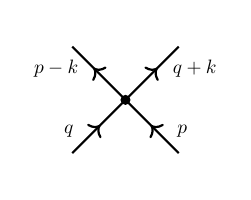
\begin{tikzpicture}[scale=.8, baseline=(current bounding box.center)]
		\node (a) at (-1, 1) {} node[scale=0.7] at (-1.1, 0.5) {$p-k$};
		\node (b) at ( 1, 1) {} node[scale=0.7] at ( 1.1, 0.5) {$q+k$};
		\node (c) at (-1,-1) {} node[scale=0.7] at (-0.9,-0.5) {$q$};
		\node (d) at ( 1,-1) {} node[scale=0.7] at ( 0.9,-0.5) {$p$};
		\begin{scope}[very thick, decoration={
				markings,
				mark=at position 0.6 with {\arrow{>}}}
			]
			\draw[black, thick, postaction={decorate}] (0,0) -- (a);
			\draw[black, thick, postaction={decorate}] (0,0) -- (b);
		\end{scope}
		\begin{scope}[very thick, decoration={
				markings,
				mark=at position 0.6 with {\arrow{<}}}
			]
			\draw[black, thick, postaction={decorate}] (0,0) -- (c);
			\draw[black, thick, postaction={decorate}] (0,0) -- (d);
		\end{scope}
		\filldraw[black] (0,0) circle (2pt); %node[anchor=west]{Intersection point};
	\end{tikzpicture}.
\end{align*}

With these we can evaluate the expectations that show up in Duhamel's formula separately. Let's start
with $\langle V \rangle_{H_0}$. This is the expectation of a sum with terms $\bar\psi\bar\psi\psi\psi$,
exactly the interaction term, and so the result will be a sum of all possible (connected) diagrams
with one vertex. Omitting the temperatures when writing two-point functions and calling
$n_k = n_\text{F}(\epsilon_k)$ the calculation is as follows:
\begin{align*}
	\langle V \rangle_{H_0}
	&= \mathbb{E}_G \biggl(
		\lambda \sum_{k,p,q} \hat{V}(k) \bar\psi_{p-k} \bar\psi_{q+k} \psi_q \psi_p
		\biggr)
	= \sum_{\Gamma \in \mathcal{G}_{\text{C},1}} \text{val}(\Gamma) \\
	&= \textcolor{red}{draw \ feynman \ diagrams} \\
	% \begin{tikzpicture}[scale=.7, baseline=(current bounding box.center)]
	% 	\node[shape=coordinate] (a) at (-1, 1) {};
	% 	\node[shape=coordinate] (b) at ( 1, 1) {};
	% 	\node[shape=coordinate] (c) at (-1,-1) {};
	% 	\node[shape=coordinate] (d) at ( 1,-1) {};
	% 	\begin{scope}[very thick, decoration={
	% 			markings,
	% 			mark=at position 0.5 with {\arrow{>}}}
	% 		]
	% 		\draw[black, thick] (0,0) -- (a);
	% 		\draw[black, thick] (0,0) -- (b);
	% 	\end{scope}
	% 	\begin{scope}[very thick, decoration={
	% 			markings,
	% 			mark=at position 0.5 with {\arrow{<}}}
	% 		]
	% 		\draw[black, thick] (0,0) -- (c);
	% 		\draw[black, thick] (0,0) -- (d);
	% 	\end{scope}
	% 	\filldraw[black] (0,0) circle (2pt); %node[anchor=west]{Intersection point};
	% 	% \draw[black, thick, postaction={decorate}] (a) .. controls (-2,-.5) and (-.5,-2) .. (d);
	% \end{tikzpicture}.
	&= \sum_{k,p,q} \hat{V}(k) G_{p-k,p}G_{q+k,q} - \sum_{k,p,q} \hat{V}(k) G_{p-k,q}G_{q+k,p} \\
	&= \sum_{k,p,q} \bigl(\hat{V}(k) \delta_{k,0} n_p n_q - \hat{V}(k) \delta_{k,p-q} n_p n_q \bigr)\\
	&= \sum_{p,q} (\hat{V}(0) - \hat{V}(p-q)) n_p n_q
\end{align*}

Let's consider the term $\langle V(\tau')V(\tau) \rangle - \langle V(\tau') \rangle\langle V(\tau) \rangle$
in the double integral now. This time we have terms with two vertices, and recalling the
linked cluster theorem the expression factorizes as follows:
\begin{align*}
	\langle V(\tau')V(\tau) \rangle - \langle V(\tau') \rangle\langle V(\tau) \rangle
	&= \mathbb{E}_G(V(\tau')V(\tau)) - \mathbb{E}_G(V(\tau'))\mathbb{E}_G(V(\tau)) \\
	&= \mathbb{E}^{\mathrm{T}}_G(V(\tau');V(\tau))\\
	&= \sum_{\Gamma\in\mathcal{G}_{\mathrm{C},2}} \mathrm{val}(\Gamma) = \star
\end{align*}

Assuming that $V$ is such that $\hat{V}(-k)=\hat{V}(k)$, the
connected diagrams with two vertices are exactly divided in two groups, up to renaming the
indices in the resulting sums. Indeed, on one hand we have diagrams that have no loops, i.e.
each vertex only has contractions with the other vertex and never with itself, and on the
other we have diagrams with two loops.

\textcolor{red}{draw the complete set of diagrams?}.

Consider the first group. Fixing an incoming and an outgoing leg on one vertex, there are 4 ways
to contract them with legs of the other vertex, and in each case there is only one way to
complete the diagram without introducing loops, therefore this group contains 4 diagrams.
For the second group, there are 4 ways to form a loop on a vertex, and given a (connected)
diagram with two vertices and two loops there exists only one way to complete it. Therefore
the second group contains 16 diagrams (all possible ways to put one loop on both vertices).
Accounting for these multiplicities, we have:
\begin{align*}
	\star &= 4 \left( \textcolor{red}{no loops} \right) + 16 \left( \textcolor{red}{with loops} \right)\\
	&= \sum_{k,p,q,k',p',q'} \hat{V}(k')\hat{V}(k) \left(
		4 \, G_{p-k,p'}G_{q'+k',q}G_{q+k,q'}G_{p'-k',p}
		+ 16 \, G_{p-k,q}G_{q+k,q'}G_{p'-k',p}G_{q'+k',p'}
	\right) \\
	&= \sum_{p,q,p'} \Bigl(
		4 \, (\hat{V}(p-p'))^2 e^{(\tau'-\tau)(\epsilon_p + \epsilon_q + \epsilon_{p'} + \epsilon_{p-p'+q})} n_p n_q n_{p'} n_{p-p'+q} \\
	&\qquad\qquad + 16 \, \hat{V}(0)\hat{V}(p-q) e^{(\tau'-\tau)(2\epsilon_p + \epsilon_q + \epsilon_{p'})} n_p^2 n_q n_{p'}
	\Bigr)
\end{align*}

Renaming some of the indices at both orders and integrating this last expression, as per
equation (\ref{eq:duhamel}), leads to the final expression of the free energy at second order

\begin{align*}
	\mathrm{log}\,\mathrm{Tr}\,e^{-\beta H}
	&= \mathrm{log}\,\mathrm{Tr}\,e^{-\beta H_0}\\
	&\quad-\beta \sum_{p,k\in\mathcal{D}_\Lambda} \left( \hat{V}(0) -\hat{V}(k) \right) n_p n_{p-k} \\
	&\quad - \sum_{p,q,k\in\mathcal{D}_\Lambda} \Biggr(
	\frac{4(\hat{V}(k))^2 n_p n_q n_{q+k} n_{p-k}}{\epsilon_p + \epsilon_q + \epsilon_{q+k} + \epsilon_{p-k}} \biggl( \beta + \frac{1 - e^{-\beta (\epsilon_p + \epsilon_q + \epsilon_{q+k} + \epsilon_{p-k})}}{\epsilon_p + \epsilon_q + \epsilon_{q+k} + \epsilon_{p-k}} \biggr) \\
	&\quad +
	\frac{16\hat{V}(0)\hat{V}(p-q) n^2_p n_q n_{p-k}}{2\epsilon_p + \epsilon_q + \epsilon_{p-k}} \biggl( \beta + \frac{1 - e^{-\beta (2\epsilon_p + \epsilon_q + \epsilon_{p-k})}}{2\epsilon_p + \epsilon_q + \epsilon_{p-k}} \biggr)
	\Biggl).
\end{align*}

Now that the computation is complete, we need to prove that removing the UV cutoff, i.e.
taking the limit $\Lambda\to\infty$, leads to a well-defined expression. Please note that this
is not at all a trivial statement and what we are doing is deciding on the order in which
to take different limits, as removing the cutoff starting from this expression means that the
perturbative series is \textit{not} done in the case where the state space is
infinite-dimensional. Physically, this does not pose any concern and we expect the two
scenarios to be equivalent, but from the point of view of mathematical rigour it is worth
pointing out this kind of subtleties.

\begin{theorem}
	With the regularity condition that, given $m\geq1$, $\partial^\alpha V\in L^1(\mathbb{T}^3)$
	for all multi-indices $\alpha$ such that $\vert\alpha\vert=m$, and the assumption that
	$\epsilon_p$ is a positive and monotonically increasing \textcolor{red}{polynomial} in
	$\vert p\vert$, the above expression converges in the limit $\Lambda\to\infty$.
\end{theorem}
\begin{proof}
	The zero-th order is trivial, as it doesn't depend on $\Lambda$ and is, in fact, finite:
	$e^{-\beta H_0}$ is trace-class and strictly positive definite, which implies
	$\vert\log\,\mathrm{Tr}\,e^{-\beta H_0}\vert<\infty$.
	Moving onto the first and second orders, by the non-stationary phase argument we can
	conclude that $\vert\hat{V}(k)\vert \leq C/\vert k\vert^m$ for some $C>0$, which means
	that at both orders the factors $\hat{V}(k)$ will be decaying as an inverse power as
	$\vert k\vert\to\infty$, which is the relevant limit as we take the cutoff $\Lambda$ to
	infinity. As for the energy terms, we are assuming that $\epsilon_k\geq0$ for all $k$, and
	that it is a monotonically increasing polynomial in $\vert k\vert$. The last factor to
	discuss is the Fermi-Dirac distribution, but this has an explicit form: an exponential
	decay in $\epsilon_k$, which leads to an explonential decay in some power (greater or
	equal to one) of $\vert k\vert$.

	With these estimates in place we can show that, in the limit $\Lambda\to\infty$, the
	expression above converges. Looking at the first order, we can write
	\begin{align*}
		\sum_{p,k\in\mathcal{D}_\Lambda} \left\vert\left(\hat{V}(0)-\hat{V}(k)\right) n_p n_{p-k}\right\vert
		&\leq \vert\hat{V}(0)\vert \sum_{p,k\in\mathcal{D}_\Lambda}n_p n_{p-k}
		+ \sum_{p,k\in\mathcal{D}_\Lambda}\vert\hat{V}(k)\vert n_p n_{p-k}\\
		&= \vert\hat{V}(0)\vert \sum_{p\in\mathcal{D}_\Lambda}n_p\sum_{k\in\mathcal{D}_\Lambda}n_{p-k}
		+ \sum_{p\in\mathcal{D}_\Lambda}n_p\sum_{k\in\mathcal{D}_\Lambda}\vert\hat{V}(k)\vert n_{p-k}.
	\end{align*}

	By the positivity of the general terms for all $k\in\mathbb{Z}^3$ we can bound the sums by
	the respective sum over $\mathbb{Z}^3$, and because the general terms of each of the above
	sums only depends on the modulus of the index we can employ the following strategy. Define
	$A_n = \{k\in\mathbb{Z}^3 : n \leq \vert k\vert < n+1\}$ and write
	\begin{align*}
		\sum_{k\in\mathbb{Z}^3} a_{\vert k\vert} = \sum_{n=0}^\infty \sum_{k\in A_n} a_{\vert k\vert}.
	\end{align*}
	Because $c_1\vert A_n\vert a_{n+1} \leq \sum_{k\in A_n}a_{\vert k\vert} \leq c_2\vert A_{n+1}\vert a_n$
	for all $n$ if $a_n$ is decreasing, and because $\vert A_n\vert\asymp n^2$, we can conclude
	that the behaviour of $\sum_{k\in\mathbb{Z}^3} a_{\vert k\vert}$ and $\sum_{n=0}^\infty n^2 a_n$
	is the same.

	Now we can show that each term converges. Indeed $\sum_{k\in\mathbb{Z}^3}n_k$ converges
	if, and only if, the series $\sum_{\ell\in\mathbb{N}} \ell^2 e^{-\beta\epsilon_\ell}$
	converges, by the asymptotic comparison test. The latter does converge absolutely as shown by
	the root test:
	\begin{align*}
		\left\vert \ell^2 e^{-\beta\epsilon_{\ell}}\right\vert^{1/\ell}
		= e^{\frac{2\log(\ell)}{\ell} - \beta\epsilon_\ell}
		\longrightarrow K \in [0,1).
	\end{align*}

	Similarly, $\sum_{k\in\mathbb{Z}^3}\vert\hat{V}(k)\vert n_k$ converges, as
	\begin{align*}
		\sum_{k\in\mathbb{Z}^3} \vert\hat{V}(k)\vert n_k
		\leq \sum_{k\in\mathbb{Z}^3}\frac{C n_k}{\vert k\vert^m}
		\leq \sum_{k\in\mathbb{Z}^3} C n_k.
	\end{align*}
	This shows that indeed the first order is, in the limit in $\Lambda\to\infty$, an
	absolutely convergent series.

	Very similar arguments can be used to show that the second order has an absolutely convergent
	series as a limit. Indeed, recalling the assumptions made about each factor present in the
	expression, we can bound the first term in the sum by
	\begin{align*}
		\sum_{p,q,k\in\mathcal{D}_\Lambda} (\ldots)
		&\leq \sum_p \frac{4n_p}{\epsilon_p} \sum_q n_q \sum_k (\hat{V}(k))^2 n_{q+k}n_{p-k}
		\left(\beta + \frac{1}{\epsilon_p}\right),
	\end{align*}
	which, turning once more sums over $\mathbb{Z}^3$ into normal series with an additional square
	in the general term, is an absolutely convergent series in the limit $\Lambda\to\infty$, as
	the only true difference from the previous case is the additional factor $1/\epsilon_p$, which
	is an inverse power and does not change the result of any of the comparison tests done before.
	The exact same argument can be applied to the second term, and this concludes the proof.
\end{proof}

And with the convergence of the free energy under control, the next step is to look at the
limit $\beta\to\infty$ to retrieve the ground state energy.

\subsection{Mean field scaling limit}

\section{On higher orders of perturbation theory}

\begin{itemize}
	\item comment on the regularity condition $\partial^\alpha\in L^1$ which excludes coulomb
		interaction;
	\item comment on third order somewhat explicitly;
	\item discuss the hope of proving that at every order $n$ the direct term $\hat{V}(k)^n$
		scales with $N^{-1/3}$;
	\item discuss difficulties in proving that the rest in duhamel's formula goes to zero
		and that non-direct terms converge.
\end{itemize}

\appendix

\section{More about operators on a Hilbert space}

We group in this appendix a series of definitions and theorems that are not necessarily part
of the basic foundations of quantum mechanics, but are still crucial in understanding how
exactly some computations are carried out and why they hold true. Some of the results
presented here go beyond the scope of our work as far as their proof is concerned, and only
serve the purpose of giving a clearer picture of what some tools actually are without having
to reference an entire course on functional analysis.

\textcolor{red}{TODO:}
\begin{itemize}
	\item introduce UNITARIES and ISOMETRIES (and talk more about self-adjoint operators?)
	\item ORTHOGONAL COMPLEMENT theorem + RIESZ representation theorem
	\item SPECTRAL theorem (which version?)
	\item DIRECT SUMS and TENSOR PRODUCTS of hilbert spaces (and their uniqueness)\\
		$\longrightarrow$ move N-fold tensor product state space definition/explanation here,
		and move construction of (anti-)symmetric tensor products into the canonical/grand
		canonical discussion, it makes more sense.
	\item INTEGRALS (and derivatives) of operator-valued functions
	\item comments on and PROPERTIES of $e^{-\beta H_0}$ (with $H_0$ bounded and maybe even
		unbounded)
	\item a couple of comments on VARIATIONAL PROBLEMS? (from blanchard maybe)
\end{itemize}

\section{On particle-hole excitations}

\textcolor{red}{How do we apply all this theory to, for example, BCS superconductors - since
Bogolubov transformations do not necessarily preserve the relations
$[a_\pm,a_\pm]_\mp = 0$ and $[a^*_\pm,a^*_\pm]_\mp = 0$ and we did rely on those too at times.}

\section{References}
\cite{test}


\cite{test}

\printbibliography

\end{document}
